\documentclass{article}

\usepackage{arxiv}

\usepackage[utf8]{inputenc} % allow utf-8 input
\usepackage[T1]{fontenc}    % use 8-bit T1 fonts
\usepackage{lmodern}        % https://github.com/rstudio/rticles/issues/343
\usepackage{hyperref}       % hyperlinks
\usepackage{url}            % simple URL typesetting
\usepackage{booktabs}       % professional-quality tables
\usepackage{amsfonts}       % blackboard math symbols
\usepackage{nicefrac}       % compact symbols for 1/2, etc.
\usepackage{microtype}      % microtypography
\usepackage{lipsum}
\usepackage{graphicx}

\title{Computer-aided Interpretable Features for Leaf Image
Classification}

\author{
    Jayani P.G. Lakshika
    \thanks{Use footnote for providing further information about author
(webpage, alternative address)---\emph{not} for acknowledging funding
agencies. Optional.}
   \\
    Department of Statistics \\
    University of Sri Jayewardenepura \\
  Nugegoda, Sri Lanka \\
  \texttt{\href{mailto:jayanilakshika76@gmail.com}{\nolinkurl{jayanilakshika76@gmail.com}}} \\
   \And
    Thiyanga S. Talagala
   \\
    Department of Statistics \\
    University of Sri Jayewardenepura \\
  Nugegoda, Sri Lanka \\
  \texttt{\href{mailto:ttalagala@sjp.ac.lk}{\nolinkurl{ttalagala@sjp.ac.lk}}} \\
  }


% Pandoc citation processing
\newlength{\csllabelwidth}
\setlength{\csllabelwidth}{3em}
\newlength{\cslhangindent}
\setlength{\cslhangindent}{1.5em}
% for Pandoc 2.8 to 2.10.1
\newenvironment{cslreferences}%
  {}%
  {\par}
% For Pandoc 2.11+
\newenvironment{CSLReferences}[3] % #1 hanging-ident, #2 entry spacing
 {% don't indent paragraphs
  \setlength{\parindent}{0pt}
  % turn on hanging indent if param 1 is 1
  \ifodd #1 \everypar{\setlength{\hangindent}{\cslhangindent}}\ignorespaces\fi
  % set entry spacing
  \ifnum #2 > 0
  \setlength{\parskip}{#2\baselineskip}
  \fi
 }%
 {}
\usepackage{calc} % for calculating minipage widths
\newcommand{\CSLBlock}[1]{#1\hfill\break}
\newcommand{\CSLLeftMargin}[1]{\parbox[t]{\csllabelwidth}{#1}}
\newcommand{\CSLRightInline}[1]{\parbox[t]{\linewidth - \csllabelwidth}{#1}}
\newcommand{\CSLIndent}[1]{\hspace{\cslhangindent}#1}

\usepackage{longtable}
\usepackage{amsmath, xparse}
\usepackage{graphicx}
\usepackage{multirow}
\usepackage{multicol}
\usepackage{booktabs}
\usepackage{subcaption}
\usepackage{caption}
\usepackage{enumitem}
\usepackage{tabularx}
\usepackage{setspace}\doublespacing
\usepackage{subfig}


\begin{document}
\maketitle

\def\tightlist{}


\begin{abstract}
Plant species identification is time consuming, costly, and requires
lots of efforts, and expertise knowledge. The studies on medicinal plant
identification are often performed based on medicinal plant leaf images.
The is because plant leaves contain a large number of diverse set of
features such as shape, veins, edge features, apices etc. that are
useful in identifying different medicinal plants. In recent, many
researchers use deep learning methods to classify plants directly using
plant images. While deep learning models have achieved a great success,
the lack of interpretability limit their widespread application. To
overcome this, we explore the use of interpretable, measurable and
computer-aided features extracted from plant leaf images. Image
processing is one of the most challenging, and crucial steps in
feature-extraction. The purpose of image processing is to improve the
leaf image by removing undesired distortion. The main image processing
steps of our algorithm involves: i) Convert original image to RGB
(Red-Green-Blue) image, ii) Gray scaling, iii) Gaussian smoothing, iv)
Binary thresholding, v) Remove stalk, vi) Closing holes, and vii) Resize
image. The next step after image processing is to extract features from
plant leaf images. We introduced 52 computationally efficient features
to classify plant species. These features are mainly classified into
four groups as: i) shape-based features, ii) color-based features, iii)
texture-based features, and iv) scagnostic features. Length, width,
area, texture correlation, monotonicity and scagnostics are to name few
of them. We explore the ability of features to discriminate the classes
of interest under supervised learning and unsupervised learning
settings. For that, supervised dimensionality reduction technique,
Linear Discriminant Analysis (LDA), and unsupervised dimensionality
reduction technique, Principal Component Analysis (PCA) are used to
convert and visualize the images from digital-image space to feature
space. All the applications are performed on Flavia and Swedish open
source benchmark leaf datasets. The results show that the features are
sufficient to discriminate the classes of interest under both supervised
and unsupervised learning settings. The results of this study are
beneficial for the researchers working in the field of developing
automated plant identification and classification systems.
\end{abstract}

\keywords{
    Medicinal
   \and
    Leaf images
   \and
    Image processing
   \and
    Feature extraction
   \and
    LDA
   \and
    PCA
  }

Keywords: Medicinal, Leaf images, Image processing, Feature extraction,
LDA, PCA

\hypertarget{introduction}{%
\section{Introduction}\label{introduction}}

~~~~~~Leaf identification is becoming very popular in classifying plant
species. Plant leaf contains significant number of features that can
help people to identify and classify the plant species. In medical
perspective, medicinal plants are usually identified by practitioners
based on years of experience through sensory or olfactory senses. The
other method of recognizing these plants involves laboratory-based
testing, which requires trained skills, data interpretation which is
costly and time-intensive. Automatic ways to identify medicinal plants
are useful especially those that are lacking experience in medicinal
plant recognition. Statistical machine learning techniques play a
crucial role in the development of automatic system to identify
medicinal plants. In developing such system input features play an
important role. The main aim of this paper is to introduce interpretable
features that can be computed based on plant leaf images. Image
processing and feature extraction play crucial roles in developing a
workflow to achieve the aim of this research.

~~~~~~The main aim of image processing is to extract important features
by removing undesired noise and distortion (Wäldchen and Mäder 2018).
Image processing steps include image segmentation (Anantrasirichai,
Hannuna, and Canagarajah 2017), image orientation, cropping, grey
scaling, binary thresholding, noise removal, contrast stretching,
threshold inversion, image normalization, and edge recognition are some
of image processing techniques applied in recent research. These steps
can be applied parallel or individually, on several times until the
quality of leaf image reaches a specific threshold.

~~~~~~The second step is feature extraction, which identifies and
encodes relevant features from leaf images (Wäldchen and Mäder 2018).
This is a challenging task due to the structural diversity of the leaf
images. Therefore, in recent years, many researchers use deep learning
methods to classify plants directly using plant images (Wu et al. 2007a;
Azlah et al. 2019; Herdiyeni and Wahyuni 2012). While deep learning
models have achieved a great success, the most models remain complex
black boxes. The lack of interpretability limit their widespread
application.

~~~~~~A digital image is a combination of pixels from three different
color planes red, green and blue. Images are stored in computers as
three separate matrices corresponding to the red, green and blue color
channels of the image. The three separate matrices corresponding to
intensities of colors at different positions of the image (Gonzalez and
Woods 2006).

~~~~~~The main aim of feature extraction is to reduce dimensionality of
this information by obtaining measurable patterns of leaf images. For
example, shape, color, and texture are some of the patterns that may be
observed. In this paper we introduce a collection of interpretable,
measurable and computer-aided features that are useful in image leaf
classification. This feature collection includes several pre-established
features identified through a thorough review of literature. Other than
existing features, we introduce a number of features computed based on
the Cartesian coordinate of the images. Furthermore, we explore the
ability of features to discriminate the class of interest under
supervised learning setting and unsupervised learning setting.

~~~~~~The paper is organized as follows. Section 2, describes about the
steps of image processing. Preprocessing is necessary before extracting
features from the images. Section 3, discusses about feature extraction
in in-detail because features are highly influenced by the plant species
to be classified. Under this section, we discuss about mainly four types
of features as shape, color, texture, and scagnostics and how to extract
them. Section 4, present empirical application. This section consists of
details about the datasets that are used to explain the applications,
and visualization of leaf images in the feature space using supervised,
and unsupervised dimensionality reduction techniques. In Section 5,
consist of summary of the software and packages that use to extract the
features. Some discussion about the outputs and concluding remarks are
given in last section.

\hypertarget{image-processing}{%
\section{Image Processing}\label{image-processing}}

~~~~~~Image processing is an essential step to reduce noise and content
enhancement while keeping its features intact. (Goyal, Kapil, and Kumar
2018). The workflow we use to process images in this paper is shown in
Figure \ref{fig:test2}. This includes seven main steps. They are: i)
converting BGR (Blue-Green-Red) image to RGB (Red-Green-Blue), ii) gray
scaling, iii) Gaussian filtering, iv) binary thresholding, v) remove
stalk, vi) close holes, and vii) image resizing. Some of these steps are
applicable only for specific images. For example, apply remove stalk is
applicable only to leaf images which has stalk.

\begin{figure}[!ht]

{\centering 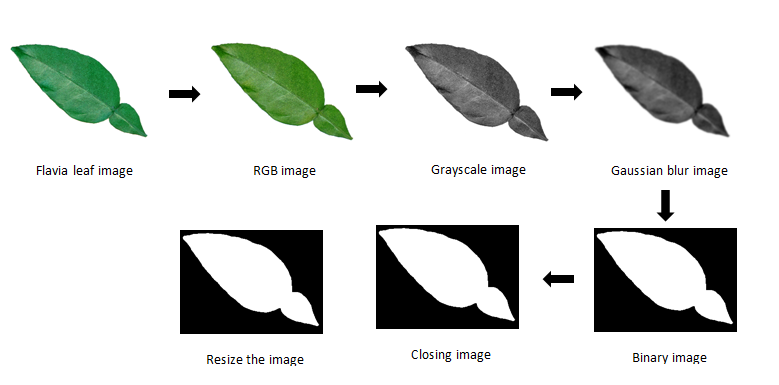
\includegraphics[width=0.5\linewidth]{/Users/thiyangashaminitalagala/Lecturer/Papers/Feature-Leaf/leaffeatures/Figures/fl5} 

}

\caption{\label{fig:test2}Image processing workflow.}\label{fig:unnamed-chunk-2}
\end{figure}

~~~~~~In this study we focus on leaves with simple arrangement as shown
in Figure \ref{simplearra}. A single leaf that is never divided into
smaller leaflet units is known as a leaf with simple arrangement. This
type of leaf is attached to a twig by its stem or the petiole. The
margins, or edges, of the leaf can be smooth, lobed, or toothed (see
Figure \ref{alledge}).

\begin{figure}[!ht]
\begin{subfigure}{.5\textwidth}
\centering
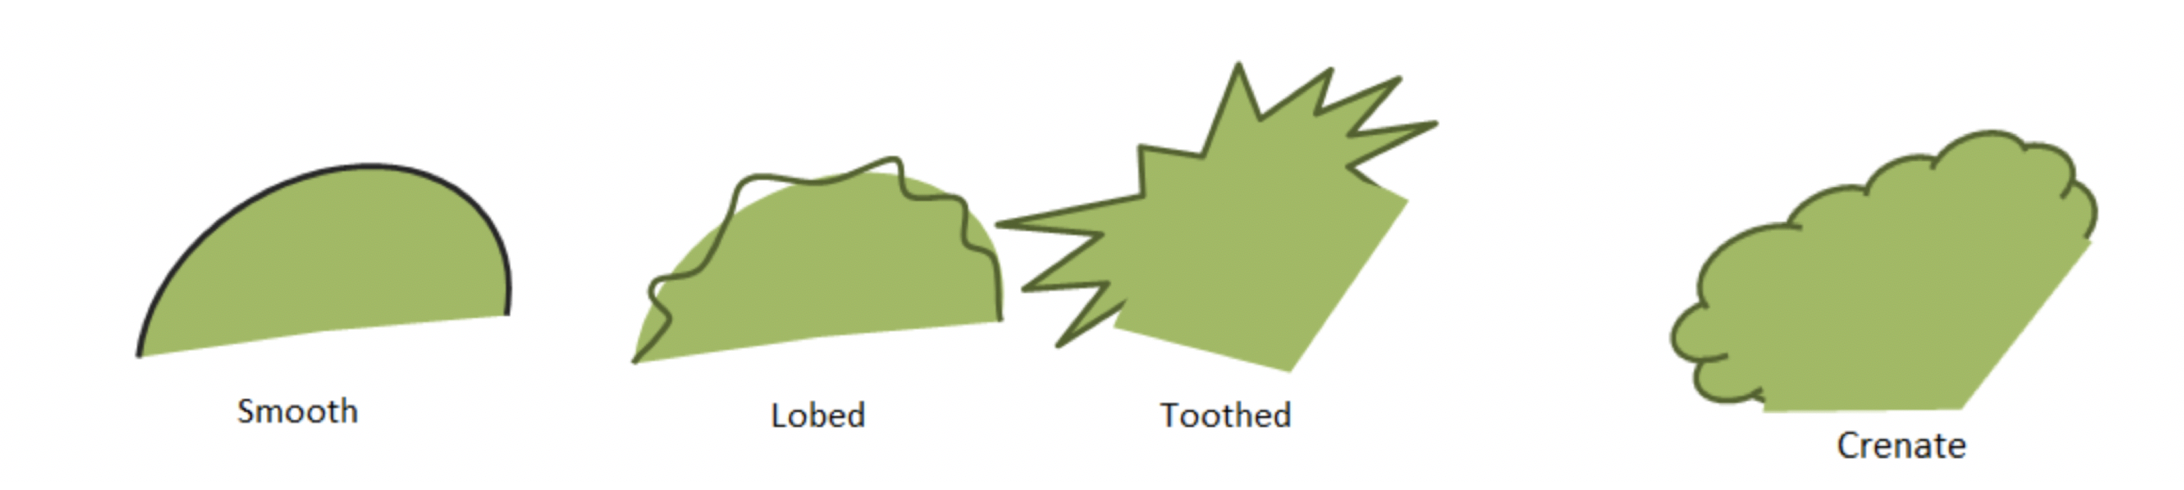
\includegraphics[width=60mm, height=50mm]{Figures/alledge.png}
        \caption{\label{alledge} Edge types of leaves focus in the study.}
\centering
        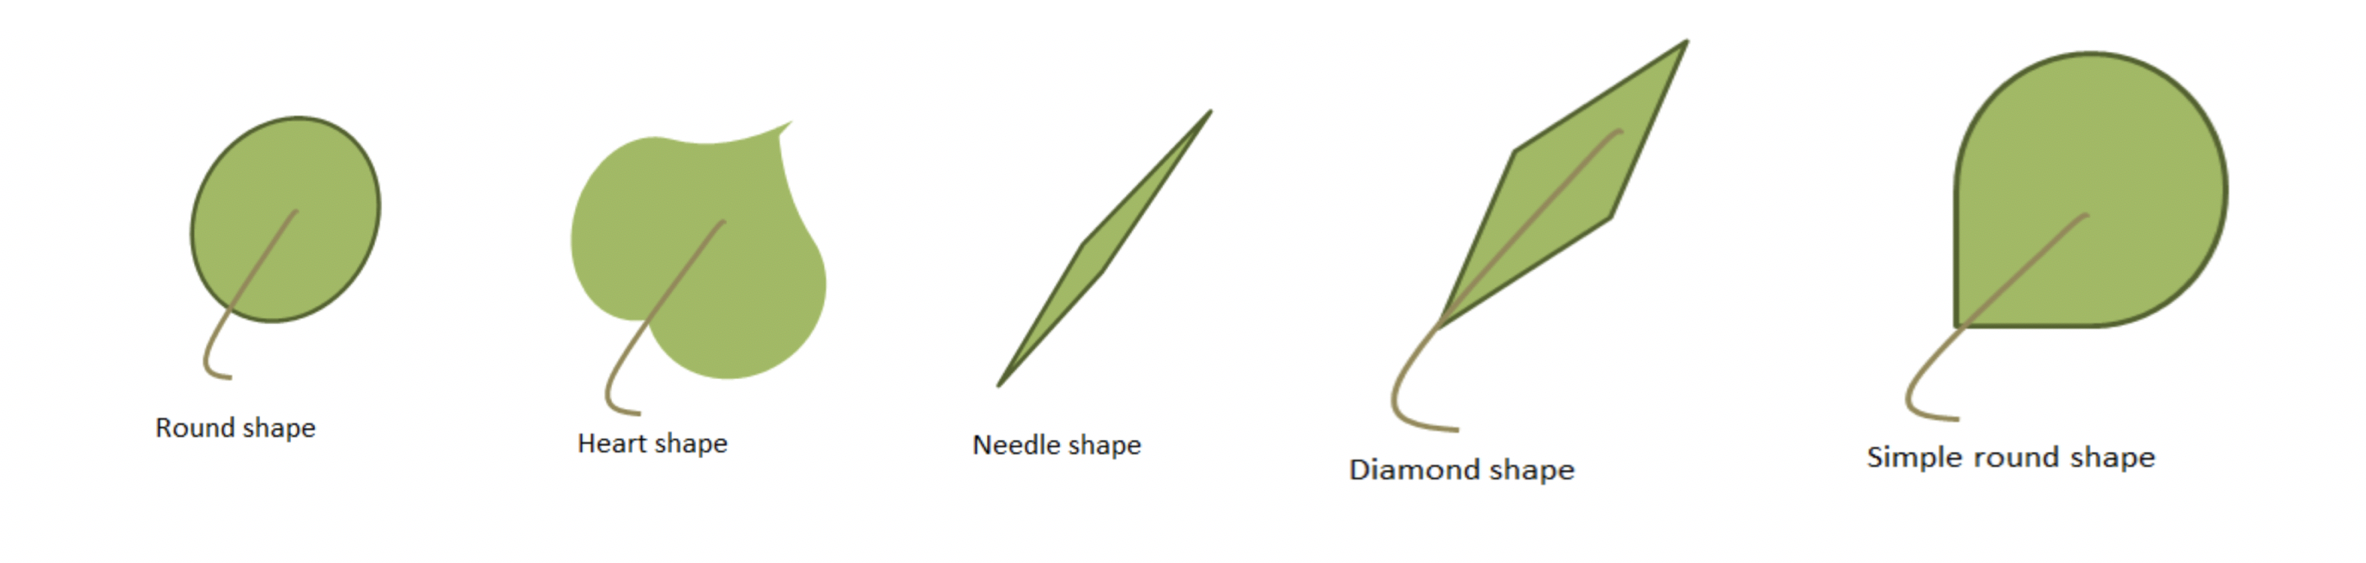
\includegraphics[width=60mm, height=50mm]{Figures/imgshape.png}
        \caption{\label{shapeimg}Shape illustrations}       
        
\end{subfigure} 
\begin{subfigure}{.5\textwidth}
\centering
        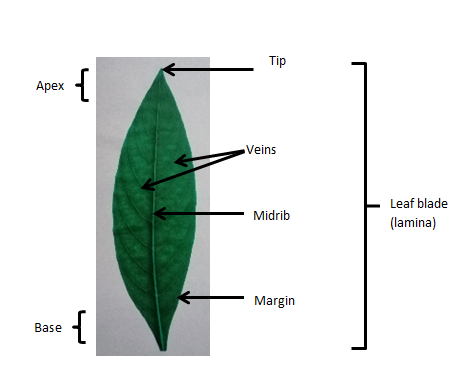
\includegraphics[width=40mm, height=30mm]{Figures/simple_leaf_parts.png}
        \caption{\label{simplearra} A leaf with simple arrangement.}
        
\end{subfigure} 

\caption{}
        \end{figure}

\hypertarget{step-1-converting-bgr-blue-green-red-image-to-rgb-red-green-blue}{%
\subsection{Step 1: Converting BGR (Blue-Green-Red) Image to RGB
(Red-Green-Blue)}\label{step-1-converting-bgr-blue-green-red-image-to-rgb-red-green-blue}}

~~~~~~BGR and RGB are conventions for the order of the different colour
channels. They are not colour spaces. When converting BGR image to RGB,
there is no any computations, just switches around the order. Several
image processing libraries have different pixel ordering. Therefore to
compatible with other libraries we convert the BGR image in to RGB
format. For an example when we read an image using OpenCV library in
Python by default it interprets BGR format, but when we plot the image
it takes the RGB format in matplotlib package in Python.

\hypertarget{step-2-grayscaling}{%
\subsection{Step 2: Grayscaling}\label{step-2-grayscaling}}

~~~~~~Grayscaling is the process of converting an image to shades of
gray from other colour spaces like RGB. This helps to increase the
contrast and intensity of images (Goyal, Kapil, and Kumar 2018). Gray
scale images require only one single byte for each pixel where as colour
(RGB) image requires 3 bytes for each pixel. Hence, grayscaling reduces
the dimension of a image.

In extracting Haralick (Haralick, Shanmugam, and Dinstein 1973) texture
features, gray-scale images are used. Another advantage of using
gray-scaled image is to reduce model complexity. Consider an example of
training neural article on RGB images of \(20 \times 20 \times 3\)
pixel. The input layer will have 1200 input nodes. Whereas for gray
scaled images the same neural network will need only 400
(\(20 \times 20\)) input node.

\hypertarget{step-3-gaussian-filtering-gaussian-blurringgaussian-smoothing}{%
\subsection{Step 3: Gaussian Filtering (Gaussian Blurring/Gaussian
Smoothing)}\label{step-3-gaussian-filtering-gaussian-blurringgaussian-smoothing}}

~~~~~~Gaussian smoothing is an image smoothing technique. Image
smoothing techniques use to remove the noise that can be occurred
because of the source (camera sensor). Image smoothing techniques help
in smoothing images and to remove low intensity edges.

~~~~~~Gaussian function is used to blur the image. It is a linear filter
which is done by using the functions in OpenCV package in Python. By
specifying the width and height of the Gaussian kernel that must be
positive and odd, and specifying the kernel standard deviation along x
and y-axis, Gaussian smoothing is established in OpenCV. When the kernel
standard deviation along x-axis is specified, kernel standard deviation
along y-axis is taken as equal to the the kernel standard deviation
along x-axis. But if both kernel standard deviation are given as zeros,
they are calculated by using the kernel size. In our research the width
and height of the kernel is defined as 55 and the kernel standard
deviation along x-axis is assigned as zero. An example of applying
Gaussian smoothing to an image is shown in Figure \ref{fig:gau}.

\begin{figure}[!ht]

{\centering 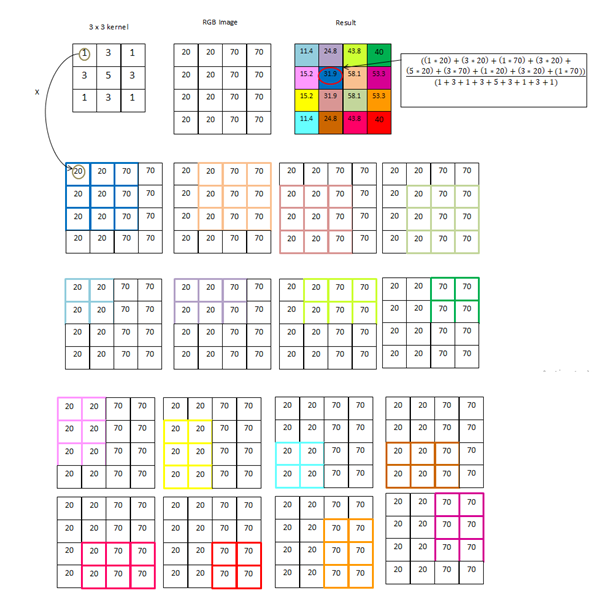
\includegraphics[width=0.6\linewidth]{/Users/thiyangashaminitalagala/Lecturer/Papers/Feature-Leaf/leaffeatures/Figures/gau} 

}

\caption{\label{fig:gau}Example of gaussian smoothing}\label{fig:unnamed-chunk-3}
\end{figure}

\hypertarget{step-4-binary-thresholding}{%
\subsection{Step 4: Binary
Thresholding}\label{step-4-binary-thresholding}}

~~~~~~Thresholding is a segmentation technique that is used to separate
foreground from its background. Thresholding converts gray-scale image
into binary image according the threshold value. If the pixel value is
smaller than the threshold value, the pixel value is set as 0, and if
not the pixel value is set to a maximum value which is generally 255.
Thersholding technique is done on grayscale images in computer vision.

~~~~~~We used Otsu's binarization (Bangare et al. (2015)) which is an
adaptive thresholding after Gaussian filtering to convert color images
to the binary images. The reason for using Otsu's binarization method
is, it automatically determines the optimal threshold value.

\textbf{Otsu's Thresholding}

~~~~~~Nobuyuki Otsu introduced Otsu's method which is defined for a
histogram of grayscale values of a histogram (\(ghist_I\)) of an input
image \(Im\). To segment an image \(Im\) into two subsets of pixels
Otsu's method calculates an optimal threshold \(\tau\). The number of
pixel locations of the gray scale image is defined as \(|\Omega|\). The
algorithm maximizes the variance \(\sigma^2\) between the two subsets
(Within-class-variance) to find the threshold \(\tau\). The variance
\(\sigma^2\) is defined as

\[\sigma^2 = P_1(\mu_1-\mu)^2 + P_2(\mu_2-\mu)^2 = P_1P_2(\mu_1-\mu_2)^2, \]

where \(\mu\) is the mean of the histogram, \(\mu_1\) and \(\mu_2\) are
the mean values of first and second subset respectively. The
corresponding class probabilities, \(P_1\) and \(P_2\) are defined as
follows,

\[P_1 = \frac{\sum_{i=0}^{u}ghist_I(i)}{|\Omega|} \text{ ,and } P_2 = \frac{\sum_{i=u+1}^{255}ghist_I(i)}{|\Omega|},\]

where \(u\) is the candidate threshold and the maximum gray level
(\(G_{max}\)) is assumed as 255. To find optimal threshold \(\tau\) for
segmenting image \(Im\), all candidate thresholds are evaluated this
way.

The algorithm of Otsu's method is defined as follows,

\begin{table}[!ht]
\centering
\begin{tabular}{l}
\hline
Create a histogram for the grayscale image \\ 
Set the histogram variance $S_{max} = 0$                                             \\ \hline
\textbf{while} $u < G_{max}$ \textbf{do}                                             \\ \hline
Compute $\sigma^2 = P_1*P_2(\mu_1-\mu_2)^2$                                             \\ 
\textbf{if} $\sigma^2 > S_{max}$ \textbf{then}                                             \\ \hline
$S_{max} = \sigma^2$                                             \\
$\tau = u$                                             \\ \hline
\textbf{end if}                                             \\ 
Set $u = u+1$                                             \\ \hline
\textbf{end while}                                             \\ \hline
\end{tabular}
\caption{Otsu's method}
\label{tab:ot}
\end{table}

~~~~~~For an example, assume that candidate threshold value \(u\) is 2.
Therefore, the image is separated into two classes, which are class 1
(\(\text{pixel value} <= 2\) ) and class 2 (\(\text{pixel value} > 2\)).
Class 1 represents the background and class 2 represents the foreground
of the grayscale image. According to Figure \ref{fig:otsu}, there are 9
pixel locations. The associated measurements are

\[P_1 = \frac{5}{9}, P_2 = \frac{4}{9}, \mu_1 = \frac{(0*2) +(1*1) + (2*2)}{(2+1+2)} = 1, \mu_2 = \frac{(3*3) +(4*1)}{(3+1)} = \frac{13}{4},\]

\[\sigma^2 = \frac{5}{9} * \frac{4}{9} * (1-\frac{13}{4})^2 = 1.25.\]

\begin{figure}[!ht]
\begin{subfigure}{.5\textwidth}
\centering
        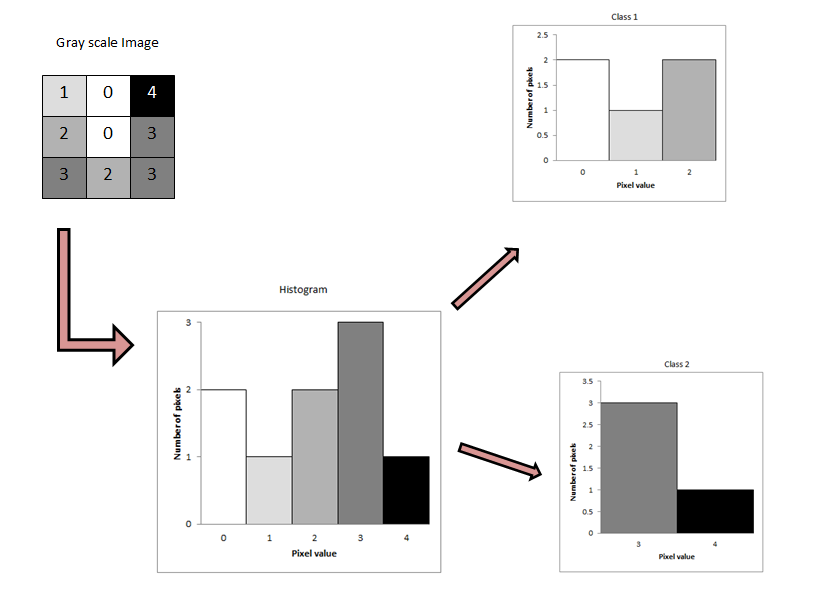
\includegraphics[width=60mm, height=50mm]{./Figures/otsu.png}
        \caption{\label{fig:otsu}Example of Otsu's binary thresholding}
        
\end{subfigure} 
\begin{subfigure}{.5\textwidth}
\centering
        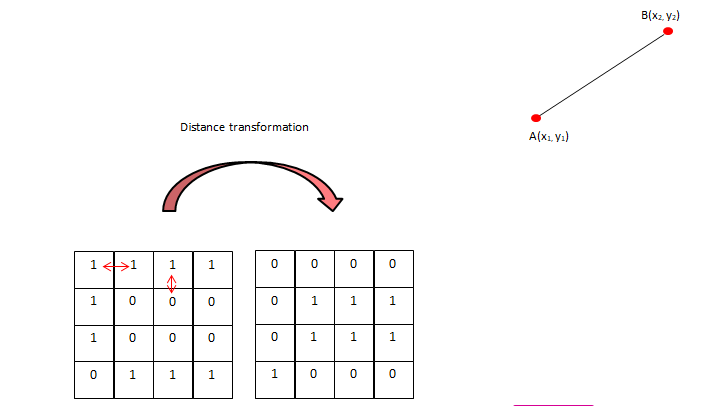
\includegraphics[width=70mm, height=60mm]{./Figures/rst.png}
        \caption{\label{fig:rstex}Example of distance transformation}
        
\end{subfigure} 

\caption{}
        \end{figure}

\hypertarget{step-5-image-resizing}{%
\subsection{Step 5: Image Resizing}\label{step-5-image-resizing}}

~~~~~~In this study we use two different benchmark leaf image datasets:
i) Flavia: 1907 fully color images of 32 classes of leaves (Wu et al.
(2007b)) and ii) Swedish: 1125 images from 15 different plant species
(Söderkvist (2001)). Flavia and Swedish images have two different image
sizes. To compare the results on different datasets, to improve the
memory storage capacity and to reduce computational complexity the leaf
images are resized to a fixed resolution. In our study, the leaf images
have been resized to {[}1600 x 1200px{]} which is the size of Flavia
leaf images.

~~~~~~Other than the main image processing techniques discussed above,
the following techniques are applied to some images where necessary
after image thresholding.

`

\begin{figure}[!ht]
\begin{subfigure}{.5\textwidth}
\centering
        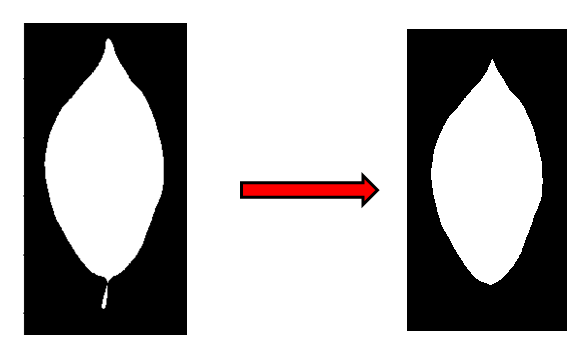
\includegraphics[width=50mm, height=40mm]{./Figures/remove_stalk.png}
        \caption{\label{fig:rst}Remove stalk}
        
\end{subfigure} 
\begin{subfigure}{.5\textwidth}
\centering
        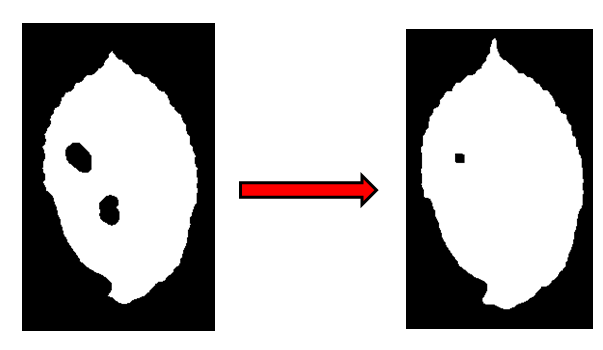
\includegraphics[width=50mm, height=40mm]{./Figures/close_holes.png}
        \caption{\label{fig:chl}Closing holes}
        
\end{subfigure} 

\caption{}
        \end{figure}

\hypertarget{remove-stalk}{%
\subsubsection{Remove Stalk}\label{remove-stalk}}

~~~~~~As shown in Figure \ref{fig:rst}, this is used to remove the stalk
of the image. Remove the petiole (stalk) of leaf image is another
version of thresholding process. Thresholding is applied after finding
the sure foreground area. To find the sure foreground area, distance
transform technique is used. Binary image is used as the input of
distance transform technique. In distance transform technique, image is
created by assigning a number for each object pixel that corresponds to
the distance to the nearest background pixel. The distance is calculated
using the Euclidean distance (see Figure \ref{fig:rstex}). After finding
the sure foreground area, Otsu's binarization is applied again as the
thresholding technique. The Euclidean distance is defined as

\begin{equation}
    \text{Euclidean distance} = \sqrt{(x_1 - x_2)^2 + (y_1 - y_2)^2.}
    \label{eu}
\end{equation}

\hypertarget{closing-holes}{%
\subsubsection{Closing Holes}\label{closing-holes}}

~~~~~~Holes inside leaf areas occur due to plant disease, light
reflection and noise. As shown in \ref{fig:chl} closing holes is used to
remove small holes inside the foreground objects. This is achieved by
pulling background pixels to foreground pixel. The closing holes is also
known as dilation and while erosion does the opposite, which is open
holes. This step is performed on a binary image.

\textbf{Erosion}

~~~~~~The basic idea of Erosion is that erodes away the boundaries of
foreground object. Since the input is binary image, a pixels in the
original image is either 1 or 0. If all the pixels under the kernel is
1, a pixel of original image is considered as 1, otherwise made to zero
(eroded). Which means that depending upon the size of the kernel all
pixels near boundary will be discarded. Therefore the thickness or size
of the foreground object decreases (White region of the image
decreases).

\textbf{Dilation}

~~~~~~Opposite of erosion is defined as dilation. If at least one pixel
under the kernel is 1, the pixel element is 1 in Dilation. It tends to
increase the foreground of the image or the white region of the object.

\hypertarget{leaf-image-features}{%
\section{Leaf Image Features}\label{leaf-image-features}}

~~~~~~In identification of plant species using leaf images, features of
leaves play an important role, because each leaf posses unique feature
that it make different from other. In previous studies (Azlah et al.
2019; Mingqiang, Kidiyo, and Joseph 2008; Sun et al. 2017), use deep
learning neural networks to classify medicinal plants based on
pixel-based images. Given the leaf images deep learning models
automatically identify features based on pixel-space of the images.
While deep learning models have achieved a great success, the lack of
interpretability of features limit their widespread application. To
overcome this, we explore the use of interpretable, measurable and
computer-aided features extracted from plant leaf images. We identified
52 features. The features are classified into four groups as: i)
shape-based features, ii) color-based features, iii) texture-based
features, and iv) scagnostic features.

\begin{figure}[!ht]

{\centering 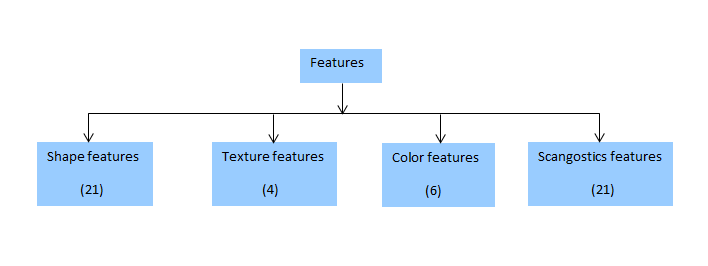
\includegraphics[width=0.7\linewidth]{/Users/thiyangashaminitalagala/Lecturer/Papers/Feature-Leaf/leaffeatures/Figures/feature_hie} 

}

\caption{\label{img33}Classification of features and their composition}\label{fig:unnamed-chunk-4}
\end{figure}

\hypertarget{shape-features}{%
\subsection{Shape Features}\label{shape-features}}

~~~~~~When identifying real-world objects, the shape is known as an
essential sign for humans. We use the shape descriptors introduced by
Wäldchen and Mäder (2018). In addition to that we introduce a number of
new shape features such as: number of convex points, x and y coordinates
of center, number of maximum and minimum points, correlation of
Cartesian contour points, etc. The shape features should be invariant to
certain class of geometric transformation of the object. The main
geometric transformation are rotation reflection, scaling and
translation (see Figure \ref{img3}). The shape features we considered in
this study are invariant to the rotation and reflection. All the shape
features are extracted from the binary images.

\begin{figure}[!ht]

{\centering 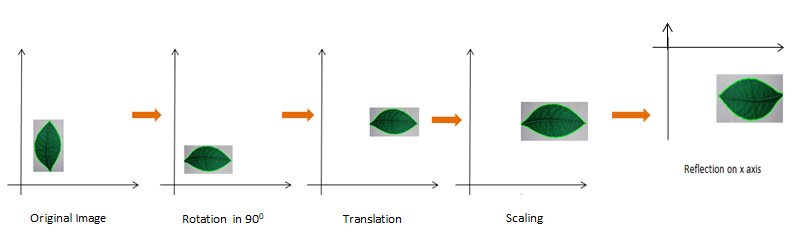
\includegraphics[width=0.7\linewidth]{/Users/thiyangashaminitalagala/Lecturer/Papers/Feature-Leaf/leaffeatures/Figures/geomatric_transformation} 

}

\caption{\label{img3} Illustration of geometric transformation}\label{fig:unnamed-chunk-5}
\end{figure}

~~~~Extraction of image contour plays an important role in measuring the
shape of a image. Simply contour (see Figure \ref{cnt}) is a curve
joining all the continuous points (along the boundary), having the same
color or intensity.

\begin{figure}[!ht]

{\centering 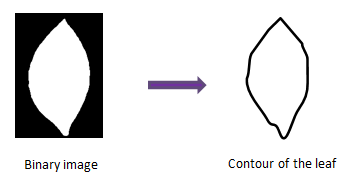
\includegraphics[width=0.3\linewidth]{/Users/thiyangashaminitalagala/Lecturer/Papers/Feature-Leaf/leaffeatures/Figures/cnt} 

}

\caption{\label{cnt}Extract contour of the leaf image}\label{fig:unnamed-chunk-6}
\end{figure}

In order to extract the contour of the leaf, the leaf should be placed
properly in the center of a white paper. If the image is place as shown
in Figure \ref{fig:trans}, as a result of inappropriate translation (a)
and inappropriate scaling (b), problems arises in the calculations of
the contour. Furthermore, it is difficult to recognize the contour, when
the image is too small.

\begin{figure}[!ht]

{\centering \subfloat[ \label{fig:trans-1}]{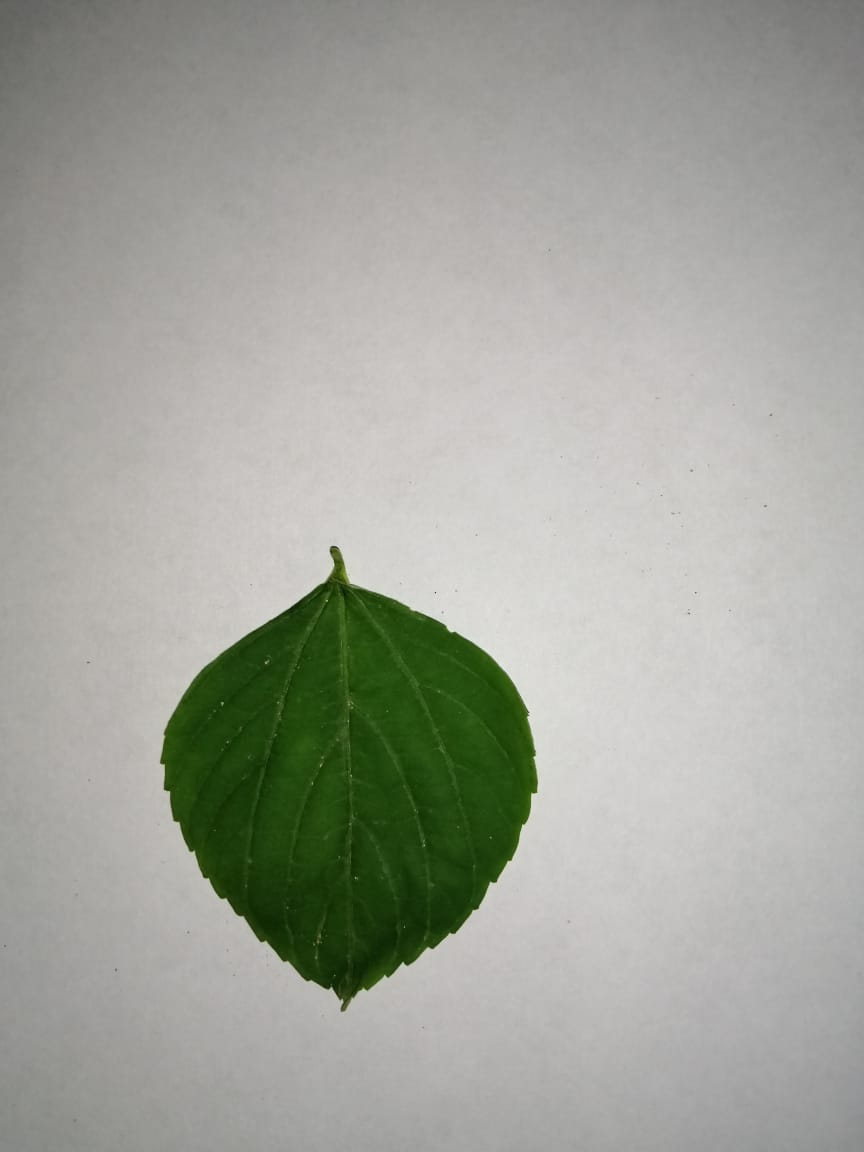
\includegraphics[width=0.1\linewidth]{/Users/thiyangashaminitalagala/Lecturer/Papers/Feature-Leaf/leaffeatures/Figures/trans} }\subfloat[\label{fig:trans-2}]{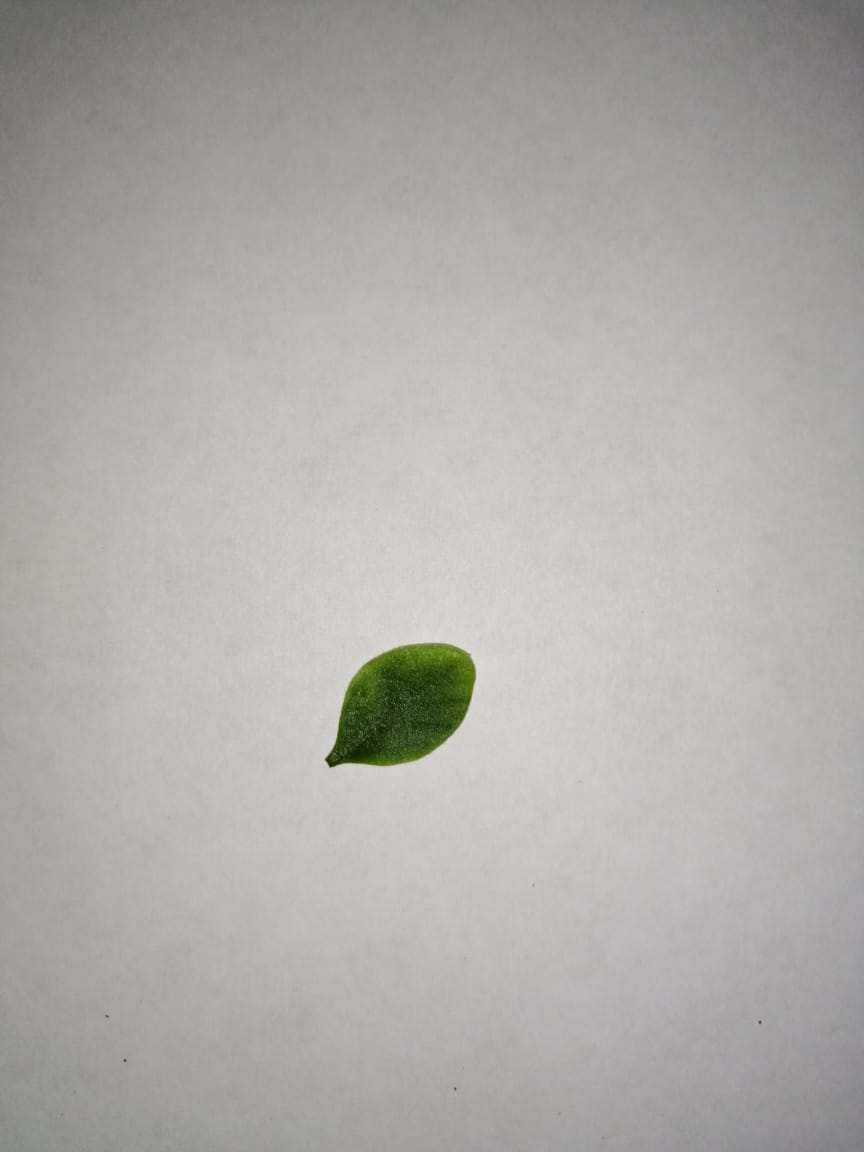
\includegraphics[width=0.1\linewidth]{/Users/thiyangashaminitalagala/Lecturer/Papers/Feature-Leaf/leaffeatures/Figures/scaling} }

}

\caption{\label{trans}Inappropriate translation (a),  Inappropriate scaling (b}\label{fig:trans}
\end{figure}

\begin{figure}[!ht]

{\centering 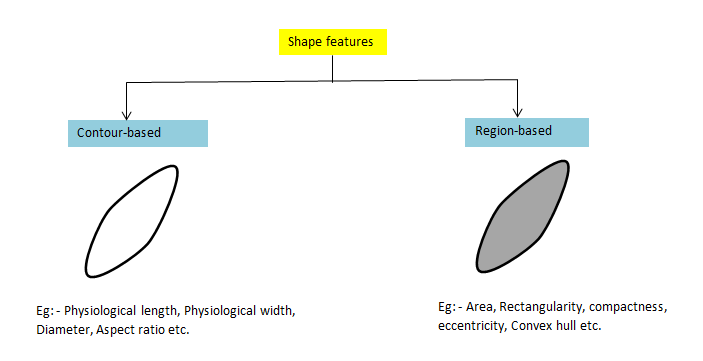
\includegraphics[width=0.6\linewidth]{/Users/thiyangashaminitalagala/Lecturer/Papers/Feature-Leaf/leaffeatures/Figures/shape_chart} 

}

\caption{\label{scalimg4}Categorization of shape features}\label{fig:unnamed-chunk-7}
\end{figure}

~~~~~~Shape features can be classified into two main categories as
contour-based and region-based features (Wäldchen and Mäder 2018). As
illustrated in Wäldchen and Mäder (2018), contour-based shape features
are computed based on the contour of a shape, whereas region-based shape
features are extracted from the whole region of a shape (see Figure
\ref{scalimg4}).

~~~~~~In this study, we use 6 initial shape features that are used to
derive 12 shape features. The 6 initial features are: i) diameter, ii)
physiological length, iii) physiological width, iv) area, v) perimeter,
and vi) eccentricity.

\hypertarget{diameter-f_1}{%
\subsubsection{\texorpdfstring{Diameter
(\(F_1\))}{Diameter (F\_1)}}\label{diameter-f_1}}

~~~~~~Diameter is defined as the longest distance between any two points
on the margin of the leaf (Wäldchen and Mäder 2018). To calculate the
diameter of the leaf image, first we need to find the contour of the
leaf image. Then we need to select all pair of contour points and
measure the Euclidean distance (equation \ref{equa_shape}) between the
two points separately. Finally, we have to find the maximum distance
among the calculated distances (see Figure \ref{shape1}). The distance
measurement is

\begin{figure}[!ht]

{\centering 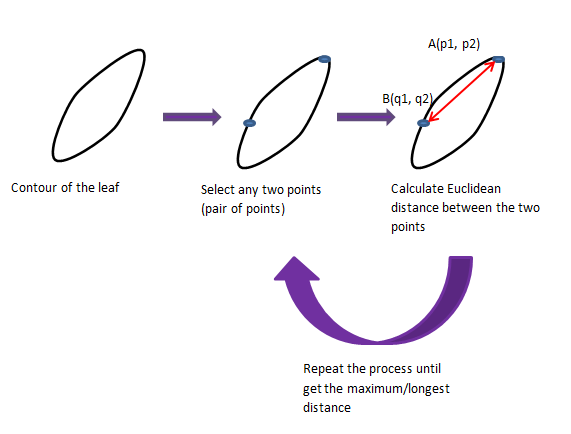
\includegraphics[width=0.5\linewidth]{/Users/thiyangashaminitalagala/Lecturer/Papers/Feature-Leaf/leaffeatures/Figures/d_cal} 

}

\caption{\label{shape1}Logic behind calculation of diameter}\label{fig:unnamed-chunk-8}
\end{figure}

\begin{equation}
    d\left( A,B\right)   = \sqrt {\sum _{i=1}^{2}  \left( q_{i}-p_{i}\right)^2},
\label{equa_shape}
\end{equation}

\begin{equation}
   F_1 = max(\sqrt{(x_i-x_j)^2 + (y_i-y_j)^2}); \forall i,j, i \neq j.
\label{equa_F1}
\end{equation}

\hypertarget{physiological-length-f_2-and-physiological-width-f_3}{%
\subsubsection{\texorpdfstring{Physiological length (\(F_2\)) and
Physiological width
(\(F_3\))}{Physiological length (F\_2) and Physiological width (F\_3)}}\label{physiological-length-f_2-and-physiological-width-f_3}}

\begin{figure}[!ht]

{\centering 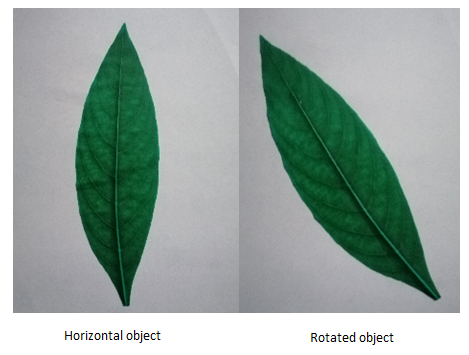
\includegraphics[width=0.2\linewidth]{/Users/thiyangashaminitalagala/Lecturer/Papers/Feature-Leaf/leaffeatures/Figures/act3} 

}

\caption{\label{act3}Straight (horizontal or vertical) and rotated leaf image in Actual leaf image dataset}\label{fig:act3}
\end{figure}

~~~~~~According to the authors in Azlah et al. (2019), the physiological
length is ``measured based on the main vein of leaf, as it stretches
from the main vein to the end tip.'' We use the definition by Azlah et
al. (2019), the physiological width is ``the span of leaf viewed from
one side to the other, from the leftmost point to the rightmost point of
leaf'' . There are straight (horizontal or vertical) and angled leaf
images in our datasets, Flavia and Swedish (see example Figure
\ref{fig:act3}). There are two types of bounding rectangles.

\begin{enumerate}
\def\labelenumi{\roman{enumi})}
\tightlist
\item
  Straight bounding rectangle: This is a straight rectangle which does
  not consider the rotation of the object (see Figure \ref{fig:act3}
  (a)).
\end{enumerate}

\begin{enumerate}
\def\labelenumi{\roman{enumi})}
\setcounter{enumi}{1}
\tightlist
\item
  Rotated rectangle: This bounding rectangle is drawn with minimum
  background area. Therefore the rotation of the object is also
  considered (see Figure \ref{fig:act3} (b)).
\end{enumerate}

The straight bounding rectangle is enough to extract physiological
length and physiological width of straight (horizontal or vertical) leaf
images. However, the straight bounding rectangle is not suitable to
compute physiological length and physiological width of angled leaf
images. To solve this problem, we considered rotated rectangle rather
than bounded rectangle in computing shape features of angled images. As
shown in Figure \ref{bound}, physiological length and width are computed
as follows:

\begin{subequations}
\begin{tabularx}{\textwidth}{Xp{3cm}X}
\begin{equation}
   F_2 = \text{Length of the rotated rectangle},
\label{equa_F2}
\end{equation}
& &
\begin{equation}
   F_3 = \text{Width of the rotated rectangle}.
\label{equa_F3}
\end{equation}

\end{tabularx}
\end{subequations}

\begin{figure}[!ht]

{\centering \subfloat[\label{fig:bound-1}]{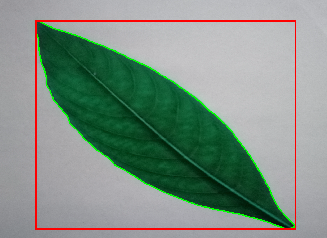
\includegraphics[width=0.3\linewidth]{/Users/thiyangashaminitalagala/Lecturer/Papers/Feature-Leaf/leaffeatures/Figures/act1} }\subfloat[\label{fig:bound-2}]{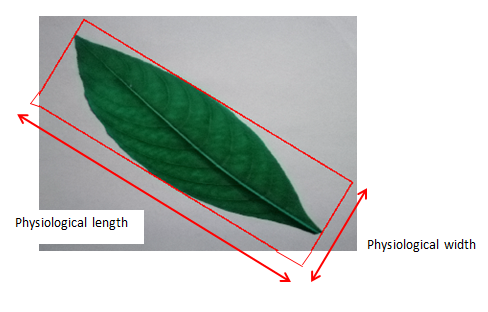
\includegraphics[width=0.3\linewidth]{/Users/thiyangashaminitalagala/Lecturer/Papers/Feature-Leaf/leaffeatures/Figures/act2} }

}

\caption{\label{bound}Straight bounded rectangle of a rotated leaf image (a), Rotated rectangle of angled leaf image (b)}\label{fig:bound}
\end{figure}

\hypertarget{area-f_4}{%
\subsubsection{\texorpdfstring{Area
(\(F_4\))}{Area (F\_4)}}\label{area-f_4}}

\begin{figure}[!ht]
\begin{subfigure}{.5\textwidth}

\centering
        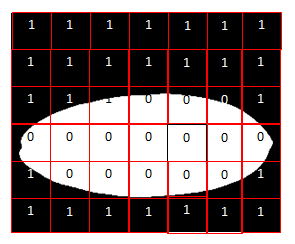
\includegraphics[width=50mm, height=40mm]{./Figures/Areacal.png}
        \caption{\label{areacal}Measure the area}
        
\centering
        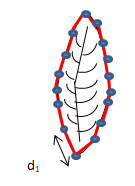
\includegraphics[width=50mm, height=40mm]{./Figures/perical.png}
        \caption{\label{calperi}Perimeter}
        
        
\end{subfigure} 
\begin{subfigure}{.5\textwidth}
\centering
        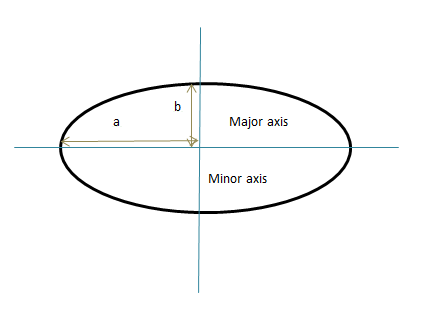
\includegraphics[width=60mm, height=50mm]{./Figures/c11.png}
        \caption{\label{shape6}Ellipse}
        
\centering
        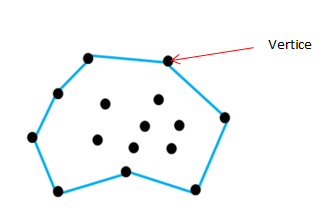
\includegraphics[width=50mm, height=40mm]{./Figures/concal.png}
        \caption{\label{shconvex}Convex hull}       
        
\end{subfigure} 

\caption{}
        \end{figure}

~~~~~~Area is computed after applying the thresholding process. Next, we
need to extract the best contour and based on that contour area is
measured. Number of 0 pixels covered by the contour is the measure of
area of leaf image (Azlah et al. 2019). As shown in Figure
\ref{areshape1} the area measures increase as the area of the leaf
increases. The area is defined by

\begin{equation}
   F_4 = \text{Number of zero pixels covered by the contour}.
\label{equa_F4}
\end{equation}

\hypertarget{perimeter-f_5}{%
\subsubsection{\texorpdfstring{Perimeter
(\(F_5\))}{Perimeter (F\_5)}}\label{perimeter-f_5}}

~~~~~As shown in Figure \ref{calperi} perimeter is defined as the
summation of euclidean distance of all continuous points in the contour.
Let \(n\) be the number of distances around the contour, then the
perimeter is defined as

\begin{equation}
   F_5 =  \sum_{i=0}^{n}d_i.
\label{equa_F5}
\end{equation}

\hypertarget{eccentricity-f_6}{%
\subsubsection{\texorpdfstring{Eccentricity
(\(F_6\))}{Eccentricity (F\_6)}}\label{eccentricity-f_6}}

~~~~~~Eccentricity is a characteristic of any conic section of a leaf
(Azlah et al. 2019). Eccentricity is defined that how much the ellipse
actually varying being circular. Eccentricity is calculated using
equation \ref{eqecc} as

\begin{equation}
    F_6 = \sqrt{1-\frac{b^2}{a^2}}.
    \label{eqecc}
\end{equation}

where \(a\) is semi-major axis and \(b\) is semi-minor axis (see Figure
\ref{shape6})

~~~~~~Eccentricity of an ellipse is varied between 0 and 1. If
eccentricity is 0, then we obtain a circle whereas eccentricity is 1,
then we obtain an ellipse (see Figure \ref{shape5}).

\hypertarget{number-of-convex-points-f_21-and-verticies}{%
\subsubsection{\texorpdfstring{Number of Convex Points (\(F_{21}\)) and
Verticies}{Number of Convex Points (F\_\{21\}) and Verticies}}\label{number-of-convex-points-f_21-and-verticies}}

~~~~~~Wilkinson, Anand, and Grossman (2005) defined a convex hull as a
``hull that contains all the straight line segments connecting any pair
of points in its interior.'' The convex hull bounds a single polygon
(see Figure \ref{shconvex}). We introduced two new features computed
based on the convex hull: i) Number of convex points (\(F_{21}\)) and
ii) Number of convex vertices (\(F_7\)).

\hypertarget{roundness-circularity}{%
\subsubsection{Roundness/ Circularity}\label{roundness-circularity}}

~~~~~~Roundness is named as aka form factor, circularity, or
isoperimetrical factor. Roundness illustrates the difference between the
leaf and a circle. Equation \ref{calround} is used to calculate
roundness. Figure \ref{shape3} visual explanation for roundness measure.
The roundness is measured by

\begin{equation}
    R = \frac{4 \pi F_4}{{F_5}^2}.
\label{calround}
\end{equation}

\hypertarget{compactness}{%
\subsubsection{Compactness}\label{compactness}}

~~~~~~Compactness is closely related to roundness. Compactness measures
that how compatible the leaf fits to a circle area (see Figure
\ref{shape4}). The compactness is measured using

\begin{equation}
    C = \frac{{F_5}^2}{F_4}.
\label{calcompact}
\end{equation}

\hypertarget{convexity}{%
\subsubsection{Convexity}\label{convexity}}

~~~~~~Convexity measures the curvature of the convex hull.

\begin{figure}[!ht]
\begin{subfigure}{.5\textwidth}

\centering
        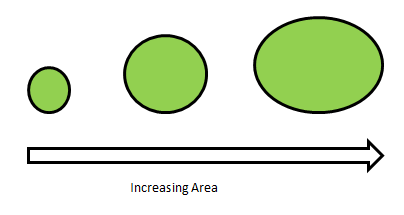
\includegraphics[width=40mm, height=30mm]{./Figures/c8.png}
        \caption{\label{areshape1}Area}

\centering
        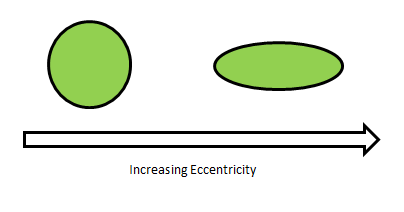
\includegraphics[width=40mm, height=30mm]{./Figures/c9.png}
        \caption{\label{shape5}Eccentricity}

\centering
        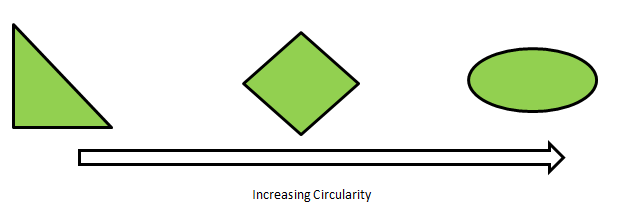
\includegraphics[width=40mm, height=30mm]{./Figures/c6.png}
        \caption{\label{shape3}Circularity}
        
\end{subfigure} 
\begin{subfigure}{.5\textwidth}

\centering
        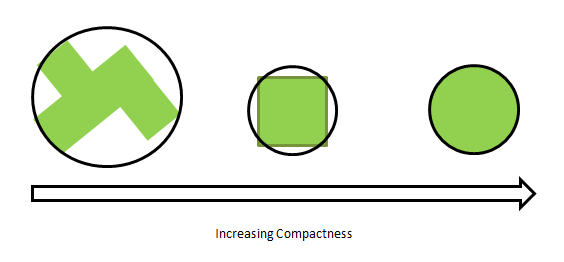
\includegraphics[width=40mm, height=30mm]{./Figures/c10.png}
        \caption{\label{shape4}Compactness}


\centering
        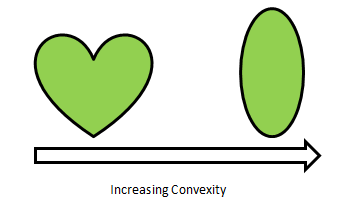
\includegraphics[width=40mm, height=30mm]{./Figures/c7.png}
        \caption{\label{shape7}Convexity}
        
\end{subfigure} 

\caption{}
        \end{figure}

The equations and software packages used to compute shape features are
shown in Table \ref{tab:table1}.

\begin{longtable}{llllll}
\hline
Shape feature        & \multicolumn{1}{c}{Feature name}                                                            & \multicolumn{1}{c}{Figure} & \multicolumn{1}{c}{Formula} & \multicolumn{1}{c}{Range} & \begin{tabular}[c]{@{}l@{}}Software \\ package\end{tabular}   \\ \hline
\endfirsthead
%
\multicolumn{6}{c}%
{{\bfseries Table \thetable\ continued from previous page}} \\
\hline
Shape feature        & \multicolumn{1}{c}{Feature name}                                                            & \multicolumn{1}{c}{Figure} & \multicolumn{1}{c}{Formula} & \multicolumn{1}{c}{Range} & \begin{tabular}[c]{@{}l@{}}Software \\ package\end{tabular}   \\ \hline
\endhead
%
\hline
\endfoot
%
\endlastfoot
%
$F_1$  & Diameter                                                                                    &  \centering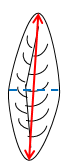
\includegraphics[width=\linewidth, height=15mm]{./Figures/diameter.png}                          & \multicolumn{1}{l}{eq:\ref{equa_F1}}        & \multicolumn{1}{l}{[0,$\infty$]}      & \begin{tabular}[c]{@{}l@{}}combinations,\\ numpy\end{tabular} \\
$F_2$                     & Physiological length                                                                        &     \centering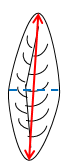
\includegraphics[width=\linewidth, height=15mm]{./Figures/Length_new.png}                       &            eq:\ref{equa_F2}                 &         [0,$\infty$)                 & OpenCV                                                        \\
$F_3$                     & Physiological width                                                                         &    \centering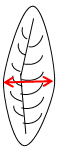
\includegraphics[width=\linewidth, height=15mm]{./Figures/width.png}                        &      eq:\ref{equa_F3}                        &           [0,$\infty$)                & OpenCV                                                        \\
$F_4$                     & Area                                                                                        &     \centering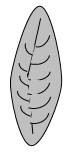
\includegraphics[width=\linewidth, height=15mm]{./Figures/area.png}                        &       eq:\ref{equa_F4}                      &                           & OpenCV                                                        \\
$F_5$                     & Perimeter                                                                                   &      \centering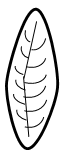
\includegraphics[width=\linewidth, height=15mm]{./Figures/perimeter.png}                      &        eq:\ref{equa_F5}                     &          [0,$\infty$)                 & OpenCV                                                        \\
$F_6$                     & Eccentricity                                                                                &                            &      eq:\ref{eqecc}                       & [0,1]                     & OpenCV                                                        \\
$F_7$, $F_8$                     & \begin{tabular}[c]{@{}l@{}}x and y coordinate \\ of center\end{tabular}                     &      \centering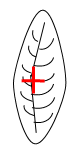
\includegraphics[width=\linewidth, height=15mm]{./Figures/centroid.png}                      &                             &                           &            scipy.ndimage                                                   \\
$F_{9}$                     & Aspect ratio                                                                                &     \centering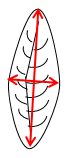
\includegraphics[width=\linewidth, height=15mm]{./Figures/AR.png}                       &       $F_9 = \frac{F_2}{F_3}$                      &       [0,$\infty$)                    &                                -                               \\
$F_{10}$                     & Roundness/ Circularity                                                                      &       \centering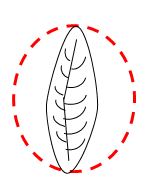
\includegraphics[width=\linewidth, height=15mm]{./Figures/roudness.png}                       &           eq:\ref{calround}                  &          [0,$\infty$)                &     numpy                                                          \\
$F_{11}$                     & Compactness                                                                                 &     \centering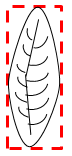
\includegraphics[width=\linewidth, height=15mm]{./Figures/rect.png}                       &        eg:\ref{calcompact}                     &     (0,$\infty$)                      &                   -                                            \\
$F_{12}$                     & Rectangularity                                                                              &                            &       $F_{12} = \frac{{F_5}^2}{F_4}$                      &      (0,$\infty$)                     &               -                                                \\
$F_{13}$                     & Narrow factor                                                                               &       \centering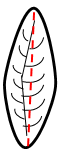
\includegraphics[width=\linewidth, height=15mm]{./Figures/nf.png}                     &         $F_{13} = \frac{F_1}{F_2}$                    &     [0,$\infty$)                      &                     -                                          \\
$F_{14}$                     & Perimeter ratio of diameter                                                                 &       \centering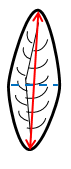
\includegraphics[width=\linewidth, height=15mm]{./Figures/pd.png}                     &         $F_{14} = \frac{F_5}{F_1}$                     &       [0,$\infty$)                    &                      -                                         \\
$F_{15}$  & \begin{tabular}[c]{@{}l@{}}Perimeter ratio \\ of physiological length\end{tabular}          &    \centering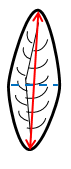
\includegraphics[width=\linewidth, height=15mm]{./Figures/pl.png}                        & $F_{15} = \frac{F_5}{F_2}$        & \multicolumn{1}{c}{[0,$\infty$)}      &         -                                                      \\
$F_{16}$  & \begin{tabular}[c]{@{}l@{}}Perimeter ratio of\\ physiological length and width\end{tabular} &    \centering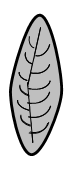
\includegraphics[width=\linewidth, height=15mm]{./Figures/plw.png}                        & $F_{16} = \frac{F_5}{F_2 * F_3}$        & \multicolumn{1}{c}{[0,$\infty$)}      &           -                                                    \\
$F_{17}$ & Perimeter convexity                                                                         &        \centering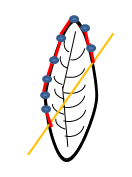
\includegraphics[width=\linewidth, height=15mm]{./Figures/p_con.png}                    & \multicolumn{1}{c}{$F_{17} = \frac{\text{Perimeter of convex hull}}{F_5}$}        & \multicolumn{1}{c}{[0,$\infty$)}      &           OpenCV                                                    \\
$F_{18}$  & Area convexity                                                                              &    \centering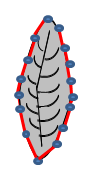
\includegraphics[width=\linewidth, height=15mm]{./Figures/a_c1.png}                         & \multicolumn{1}{c}{$F_{18} = \frac{(\text{Area of convex hull}-F_4)}{F_4}$}        & \multicolumn{1}{c}{[0,$\infty$)}      &               OpenCV                                                \\
$F_{19}$  & Area ratio of convexity                                                                     &     \centering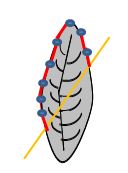
\includegraphics[width=\linewidth, height=15mm]{./Figures/a_c2.png}                        & $F_{19} = \frac{F_4}{\text{Area of convex hull}}$        & \multicolumn{1}{c}{[0,$\infty$)}      &               OpenCV                                                \\
$F_{20}$  & Equivalent diameter                                                                         &    \centering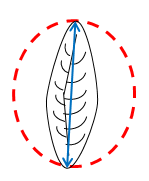
\includegraphics[width=\linewidth, height=15mm]{./Figures/eq_d.png}                        & \multicolumn{1}{c}{$F_{20} = \sqrt{\frac{4*F_4}{\pi}}$}        & \multicolumn{1}{c}{[0,$\infty$)}      &      numpy                                                         \\
\multicolumn{1}{l}{$F_{21}$} & \begin{tabular}[c]{@{}l@{}}Number of \\ convex points\end{tabular}                          &    \centering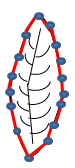
\includegraphics[width=\linewidth, height=15mm]{./Figures/convex.png}                        & number of convex points        & \multicolumn{1}{c}{[0,$\infty$)}      & OpenCV                                                        \\ \hline
\caption{Summary of shape features.}
\label{tab:table1}\\
\end{longtable}

\hypertarget{texture-features}{%
\subsection{Texture Features}\label{texture-features}}

~~~~~~Texture features are used to describe the surface or the
appearance of the leaf image. Texture can be assessed using a group of
pixels. Color is a property of a pixel. Texture is defined as feel of
various materials to human touch and texture is quantified based on
visual interpretation of this feeling. Leaf surface is a natural texture
which has random persistent patterns and do not show detectable
quasi-periodic structure (Wäldchen and Mäder 2018). Therefore to
describe the natural texture patterns of the leaf fractal theory
(Wäldchen and Mäder 2018) is the best approach.\\
\hspace*{0.333em}\hspace*{0.333em}\hspace*{0.333em}\hspace*{0.333em}\hspace*{0.333em}\hspace*{0.333em}The
Haralick texture features (Dean 1999) are functions of the normalized
GLCM (Gray Level Co-occurrence Matrix) which is a common method to
represent image texture.

\[GLCM = \begin{bmatrix}
h(1,1) & h(1,2)  & \cdot &\cdot &\cdot & h(1,n) \\ 
h(2,1) & h(2,2)  & \cdot &\cdot &\cdot & h(2,n) \\ 
\cdot  & \cdot & \cdot  & & &\cdot\\ 
\cdot  & \cdot &  & \cdot& &\cdot\\ 
\cdot  & \cdot &  & & \cdot &\cdot\\ 
h(n,1) & h(n,2) & \cdot &\cdot &\cdot & h(n,n)
\end{bmatrix}\]

~~~~~~The GLCM is square with dimension \(n\), where \(n\) is the number
of gray levels in the image. Let \(h(a,b)\) is the probability that a
pixel with value \(a\) will be found adjacent to a pixel of value \(b\).
Then \(h(a,b)\) is defined as

\[h(a,b) = \frac{\text{Number of times a pixel with value a is adjacent to a pixel with value b}}{\text{Total number of such comparisons made}}.\]

~~~~~~In order to calculate \(h(a,b)\), adjacency can be defined to
occur in each of four directions in a 2D (see Figure \ref{img2}), square
pixel image (horizontal, vertical, left and right diagonals - see
equation \ref{direction}).

\begin{figure}[!ht]

{\centering 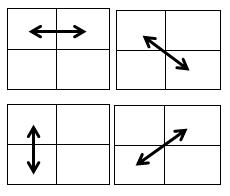
\includegraphics[width=0.2\linewidth]{/Users/thiyangashaminitalagala/Lecturer/Papers/Feature-Leaf/leaffeatures/Figures/GLMC_direction} 

}

\caption{\label{direction}Four directions of adjacency as defined for calculation of the Haralick texture features}\label{fig:unnamed-chunk-9}
\end{figure}

~~~~~~The Haralick statistics (Dean 1999) are calculated based on the
matrices generated using each of these directions (see Figure
\ref{img1}) of adjacency. Haralick introduced 14 statistics to describe
the texture of the image based on the four co-occurrences matrices
generated. In this research, we only used the following 4 statistics
among 14 of them, because most of the researchers used these 4
statistics as texture features (see Figure \ref{tabmytable}) of leaf
images. All the texture features are extracted from the gray scale
image. Texture features are calculated from the mahotas package in
Python. Table \ref{tabmytable} shows the definitions of texture
features.

\begin{table}[!ht]
\resizebox{\textwidth}{!}{%
\begin{tabular}{cclcc}
\hline
Texture feature & Feature name                                                             & \multicolumn{1}{c}{\begin{tabular}[c]{@{}c@{}}Detailed \\ description\end{tabular}}                                                                                                                       & Formula & Value range \\ \hline
    $F_{22}$            & Contrast                                                                 & \begin{tabular}[c]{@{}l@{}}Measures the\\ relation or difference\\ between the highest and\\ lowest gray levels of the GLCM\end{tabular}                                                                  &   $\frac{\sum_{a=1}^{columns}\sum_{b=1}^{rows}(a-b)^2 h(a,b)}{\text{Number of gray levels}-1}$      &     [0,$\infty$]        \\
     $F_{23}$           & Entropy                                                                  & \begin{tabular}[c]{@{}l@{}}Measures the randomness which means\\ that how uniform the image is\end{tabular}                                                                                               &    $-\sum_{a=1}^{columns}\sum_{b=1}^{rows}h(a,b)log_2(h(a,b))$     &    [$-\infty$,0]         \\
      $F_{24}$          & Correlation                                                              & \begin{tabular}[c]{@{}l@{}}Measurement of dependence\\ of gray levels of the GLCM. \\ It measures that how a particular\\ pixel is correlated to it's neighbor pixel\\ over the whole image\end{tabular} &  $\frac{\sum_{a=1}^{columns}\sum_{b=1}^{rows}(ab)h(a,b)-\mu_{x}\mu _{y}}{\sigma _{x}\sigma _{y}}$       &    [-1,1]         \\
      $F_{25}$          & \begin{tabular}[c]{@{}c@{}}Inverse \\ difference \\ moments\end{tabular} & \begin{tabular}[c]{@{}l@{}}It's a measure of homogeneity.\\ Inverse level of contrast that measures \\ how close the values of GLCM to\\ diagonal values in GLCM\end{tabular}                             &   $\sum_{a=1}^{columns}\sum_{b=1}^{rows}\frac{h(a,b)}{(a-b)^2}$      &     [0,$\infty$]        \\ \hline
\end{tabular}%
}
\caption{Definitions of texture features}
\label{tabmytable}
\end{table}

Let \(h(a, b)\) = Probability density function of gray - level pairs
\((a,b)\) and dimension of GLCM is \(n \times n\)
(\(\text{Number of columns} \times \text{Number of rows}\)). The
associated measures are given by

\[\mu_{x} = \sum_{a=1}^{columns}a\sum_{b=1}^{rows}h(a,b), \mu_{y} = \sum_{b=1}^{rows}b\sum_{a=1}^{columns}h(a,b),\]

\[\sigma_{x} = \sum_{a=1}^{columns}(a-\mu_{x})^2\sum_{b=1}^{rows}h(a,b), \sigma_{y} = \sum_{b=1}^{rows}(b-\mu_{y})^2\sum_{a=1}^{columns}h(a,b).\]

\begin{figure}[!ht]

{\centering 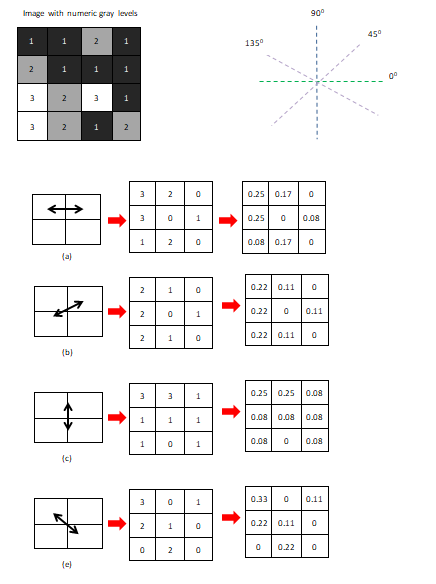
\includegraphics[width=0.5\linewidth]{/Users/thiyangashaminitalagala/Lecturer/Papers/Feature-Leaf/leaffeatures/Figures/GLMC1} 

}

\caption{\label{img1}Computing the Haralick texture features from a 4 × 4 example image step by step}\label{fig:unnamed-chunk-10}
\end{figure}

\begin{figure}[!ht]

{\centering 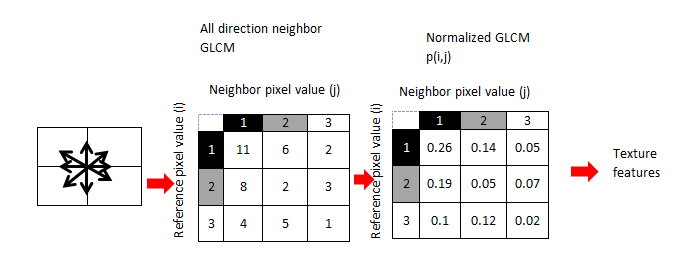
\includegraphics[width=0.5\linewidth]{/Users/thiyangashaminitalagala/Lecturer/Papers/Feature-Leaf/leaffeatures/Figures/GLMC2} 

}

\caption{\label{img2}Computing the Haralick texture features from a 4 × 4 example image with all direction}\label{fig:unnamed-chunk-11}
\end{figure}

\hypertarget{color-features}{%
\subsection{Color Features}\label{color-features}}

\begin{figure}[!ht]

{\centering 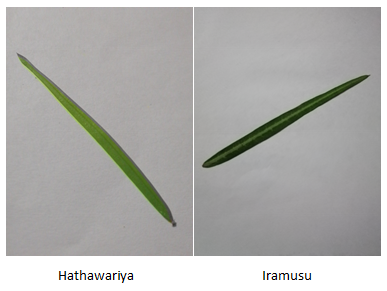
\includegraphics[width=0.3\linewidth]{/Users/thiyangashaminitalagala/Lecturer/Papers/Feature-Leaf/leaffeatures/Figures/leaf_img} 

}

\caption{\label{leafimg} Images of plant species Hathawariya and Iramusu.}\label{fig:unnamed-chunk-12}
\end{figure}

~~~~~~Color is an important characteristic of images (Wäldchen and Mäder
2018; Caglayan, Guclu, and Can 2013). Some of leaf images have very
similar shape like Hathawariya (Figure \ref{leafimg}) and Iramusu
(Figure \ref{leafimg}). Even though shapes are similar in some leaves,
there are some differences in colors of leaf images. Therefore in
addition to the shape features, we extract features related to the
color. Colors of an image are formed based on Red-Green-Blue (RGB)
colour channels of an image. Color properties are defined within a
particular color channel (Kodituwakku and Selvarajah 2004; Wäldchen and
Mäder 2018). In the field of image recognition, a number of general
color descriptors have been introduced. Color moments (Kodituwakku and
Selvarajah 2004; Wäldchen and Mäder 2018) are the simple descriptor
among them. Mean, standard deviation skewness and kurtosis are the
common moments. Color moments are convenient for real-time applications
due its low dimension and low computational complexity.

~~~~~~We used mean(\(M\)) and standard deviation(\(SD\)) of intensity
values of red, green and blue channels as color features. Let \(h\) be
the number of pixels of the image and \(r\) is the channel type which
can be red, green, or blue. The corresponding colour features are
calculates as follows:

\begin{equation}
    M = \frac{\text{Total insensity value of } r^{th} \text{channel of the image pixels}}{\text{Total intensity value of the image}},
\label{equa2}
\end{equation}

\begin{equation}
    SD = \frac{\sqrt{\sum_{j=0}^{h}(r^{th} \text{channel intensity}_j - r^{th} \text{mean value})^2}}{\text{Total intensity value of the image}}.
\label{equa3}
\end{equation}

\hypertarget{scagnostic-features}{%
\subsection{Scagnostic features}\label{scagnostic-features}}

~~~~~~Scagnostic features are used to quantify the characteristics of 2D
scatterplot diagrams (Wilkinson and Wills (2008)). Scagnostic measures
are calculated based on the appearance of scatterplot. All the
scagnostics features are calculated by using the R package called
\texttt{binostics}. Scagnostic features has the range of {[}0,1{]}.
There are 9 measures which are classified into three categories as shown
in Figure \ref{scagimg}. Based on binary images, scagnostic features are
extracted. To the best of our knowledge this is the first time, the
scagnostic features are used for image recognition.

\begin{figure}[!ht]

{\centering \includegraphics[width=0.7\linewidth]{/Users/thiyangashaminitalagala/Lecturer/Papers/Feature-Leaf/leaffeatures/Figures/scag} 

}

\caption{\label{scagimg}Hierarchy of Scagnostics}\label{fig:unnamed-chunk-13}
\end{figure}

~~~~~~~We separately measure the scagnostic features based on cartesian
and polar coordinate of the contour (see Figure \ref{pc}). As the first
step, we have to extract the contour of the leaf image (see Figure
\ref{scp}). Then find the \(x\) and \(y\) coordinate values of the
cartesian and polar separately. The \(x\) and \(y\) coordinate value is
used to calculate the scagnostic features. The following definitions can
be useful in understanding scagnostics features.

\begin{figure}[!ht]
\begin{subfigure}{.5\textwidth}
\centering
        \includegraphics[width=60mm, height=50mm]{./Figures/pc.png}
        \caption{\label{pc}Polar coordinate}
        
\end{subfigure} 
\begin{subfigure}{.5\textwidth}
\centering
        \includegraphics[width=60mm, height=50mm]{./Figures/scp.png}
        \caption{\label{scp}Preprocessing for Scagnostics}
        
\end{subfigure} 

\caption{}
        \end{figure}

\textbf{Geometric Graphs}

\begin{enumerate}
\def\labelenumi{\roman{enumi})}
\item
  Graph: A graph \(Gr = (Ve, Ed)\) is defined as a set of vertices
  (\(Ve\)) together with a relation on \(Ve\) induced by a set of edges
  (\(Ed\)). A pair of vertices is defined as an edge \(e(\nu,\omega)\),
  with e \(\in\) Ed and \(\nu,\omega \in\) Ve.
\item
  Geometric Graph: A geometric graph \(G* = [f(Ve), g(Ed), S]\); is an
  mapping of vertices to points and edges to straight lines to connect
  points in a metric space \(S\).
\end{enumerate}

\begin{enumerate}
\def\labelenumi{\roman{enumi})}
\setcounter{enumi}{2}
\item
  Length of an edge: The Euclidean distance between vertices that
  connected to edge is defined as the length of an edge, \(length(e)\).
\item
  Length of a graph: The sum of the lengths of edges in graph is known
  as the length of a graph, \(length(Gr)\).
\item
  Path: A list of successively adjacent, distinct edges are known as a
  path. If first and last vertices coincide, then the path is closed.
\item
  Polygon: A region bounded by a closed path is known as a polygon
  (\(P\)). A polygon bounded by exactly one closed path with no
  intersecting edges is known as a simple polygon.
\item
  Perimeter of a simple polygon: The length of boundary of a simple
  polygon is known as the perimeter of a simple polygon. The area of
  interior of a simple polygon is known as the area of a simple polygon.
\end{enumerate}

\begin{figure}[!ht]
\begin{subfigure}{.5\textwidth}
\centering
        \includegraphics[width=60mm, height=50mm]{./Figures/c4new.png}
        \caption{\label{scagimg5}Graph with 5 vertices and 5 edges}

\centering
        \includegraphics[width=60mm, height=50mm]{./Figures/c5.png}
        \caption{\label{scagimg4}Convex hull and alpha hull}
        
\end{subfigure} 
\begin{subfigure}{.5\textwidth}
\centering
        \includegraphics[width=60mm, height=50mm]{./Figures/c3.png}
        \caption{\label{scagimg6}Vertices of degree 2}
        
\end{subfigure} 

\caption{}
        \end{figure}

The calculation of scagnostic features require identification of the
minimum spanning tree, convex hull and alpha hull.

\textbf{Minimum Spanning Tree:}

The spanning tree of the graph is defined as \(G'(V',E')\), where
\(V' = Ve\), \(E' \subset Ed\) and \(E' = |Ve|-1\). A graph can have
more than one spanning tree. Spanning tree should not be disconnected
and should not contain any cycles. A spanning tree whose total length is
least of all spanning trees on a given set of points is known as a
Minimum Spanning Tree (MST).

\textbf{Convex hull and Alpha hull}

\begin{enumerate}
\def\labelenumi{\roman{enumi})}
\tightlist
\item
  Convex Hull (see Figure \ref{scagimg4}): Given a set of points
  embedded in 2D Euclidean space, the convex hull of the set is the
  smallest convex polygon that contains all the points of it.
\end{enumerate}

\begin{enumerate}
\def\labelenumi{\roman{enumi})}
\setcounter{enumi}{1}
\tightlist
\item
  Alpha Hull (see Figure \ref{scagimg4}): The alpha hull is a
  generalization of the convex hull. It is defined as the union of all
  convex hulls of the input within balls of radius alpha. In otherwords,
  it is a set of piecewise linear simple curves in the Euclidean plane
  associated a given set of points in the 2D Euclidean space. An open
  disk (\(D(r)\)) with radius \(r\) is used to define the indicator
  function to identify the associated points. If a point is on the
  boundary of \(D\) then \(D\) \textit{touches} a point and if a point
  is inside \(D\) then \(D\) \textit{contains} a point.
\end{enumerate}

\hypertarget{preprocessing-steps-related-to-scagnostic-features}{%
\subsubsection{Preprocessing steps related to scagnostic
features}\label{preprocessing-steps-related-to-scagnostic-features}}

~~~~~~~~~~To improve the performance of the algorithm and robustness of
the measures, preprocessing techniques such as binning and deleting
outliers are used before computing geometric graphs related features.

\begin{enumerate}
\def\labelenumi{\roman{enumi})}
\tightlist
\item
  Binning
\end{enumerate}

~~~~~~As the first step of binning, the data are normalized to the unit
interval. Then use a \(40 \times 40\) hexagonal grid to aggregate the
points in each scatterplot. We reduce the bin size by half and rebind
until no more than 250 non-empty cells. If there are more than 250
non-empty cells. When selecting the bins two important points to
consider are: i) efficiency (too many bins slow down calculations of the
geometric graphs) and ii) sensitivity (fewer bins obscure features in
the scatterplots). To improve the performance, hexagon binning is used.
To manage the problem of having to many points that start to overlap,
hexagon binning is used. The plots of hexagonal binning are density
rather than points. There are several reasons for using hexagon binning
instead of square binning in a 2D surface. Hexagons are more similar to
circle than square. To keep scagnostics orientation-independent this
bias reduction is important.

The weight function is defined as

\begin{equation}
    \text{weight} = 0.7 + \frac{0.3}{1 + t^2},
    \label{w2}
\end{equation}

where \(t=\frac{n}{500}\). (\(n\) is the number of vertex)

~~~~~~~If \(n > 2000\) then this function is fairly constant. By using
hex binning the shape and the parameters of the function is determined.
In computing sparse, skewed and convex scagnostics this weight function
is used to adjust for bias.

\begin{enumerate}
\def\labelenumi{\roman{enumi})}
\setcounter{enumi}{1}
\tightlist
\item
  Deleting Outliers
\end{enumerate}

~~~~~~To improve robustness of the scagnostics, deleting outliers can be
used. A vertex whose adjacent edges in the MST all have a weight
(length) greater than \(\omega\) is defined as an outlier in this
context. By considering nonparametric criterion for the simplicity and
Tukey's idea choose the following weight calculation is

\begin{equation}
    \text{weight} = qu_{75} + 1.5(qu_{75} - qu_{25}),
    \label{w1}
\end{equation}

where \(qu_{75}\) is the 75th percentile of the MST edge lengths and
\((qu_{75} - qu_{25})\) is the interquartile range of the edge lengths.

\begin{enumerate}
\def\labelenumi{\roman{enumi})}
\setcounter{enumi}{2}
\tightlist
\item
  Degree of a Vertex
\end{enumerate}

~~~~~~~The degree of a vertex in an undirected graph is the number of
edges associated with the vertex. For example, vertices of degree 2
means there are 2 edges associated with each vertex (see Figure
\ref{scagimg6}).

\hypertarget{definitions-of-scagnostic-features}{%
\subsubsection{Definitions of Scagnostic
Features}\label{definitions-of-scagnostic-features}}

~~~~~~The definitions of scagnostic features are defined as follows. Our
notations are as follows: i) Convex hull (\(CH\)), ii) Alpha hull
(\(Al\)) and iii) Minimum spanning tree (\(MST\)). In the following
section we give a brief description of the calculation of scagnostic
measures. For more details on rotation techniques, see Wilkinson and
Wills (2008).

\hypertarget{density-measures}{%
\subsubsection{Density Measures}\label{density-measures}}

\begin{enumerate}
\def\labelenumi{\roman{enumi})}
\tightlist
\item
  Outlying: The outlying measure is calculated before deleting the
  outliers for the other measures. The outlying measure is
\end{enumerate}

\begin{equation}
      F_{sc1} = \frac{\text{Total length of edges adjacent to outlying points}}{\text{Total edge length of the MST}}.
\end{equation}

\begin{enumerate}
\def\labelenumi{\roman{enumi})}
\setcounter{enumi}{1}
\tightlist
\item
  Skewed: The skewed measure is the first measure of relative density
  which is a relatively robust measure of skewness in the distribution
  of edge lengths. After adaptive binning skewed tends to decrease with
  \(n\). The skewed measure is calculated using the equations
\end{enumerate}

\begin{equation}
    F_{sc2} = 1-\text{weight}*(1-qu_{skew}), 
\end{equation}

~~~~~~where,

\begin{equation}
    qu_{skew} = \frac{qu_{90}-qu_{50}}{qu_{90}-qu_{10}}, 
\end{equation}

~~~~~~~and the calculation of \(weight\) is given in equation \ref{w2}.

\begin{enumerate}
\def\labelenumi{\roman{enumi})}
\setcounter{enumi}{2}
\tightlist
\item
  Sparse: The second relative density measure is sparse measure that
  measures whether points in a 2D scatterplot are confined to a lattice
  or a small number of locations on the plane. The sparse is measured by
\end{enumerate}

\begin{equation}
   F_{sc3} = \text{weight} *qu_{90},
\end{equation}

~~~~~~~where the weight function is equation \ref{w2} and \(qu_{90}\) is
the 90th percentile of the distribution of edge lengths in the \(MST\).

~~~~~~~The \(\alpha\) statistic exceeds unity (e.g., when all points
fall on either of the two diagonally opposing vertices of a square),
clamp the value to 1 in the extremely rare event Wilkinson, Anand, and
Grossman (2005).

\begin{enumerate}
\def\labelenumi{\roman{enumi})}
\setcounter{enumi}{3}
\tightlist
\item
  Clumpy: Clumpiness measures the amount of small-scale structures in
  the 2D-scatter plot (Wilkinson and Wills 2008). In order to calculate
  this feature another measurement called \(T\) is needed which is
  calculated based on RUNT graph (Hartigan and Mohanty 1992). The clumpy
  is measured by
\end{enumerate}

\begin{equation}
    F_{sc4} = max_j[1-\frac{max_k[length(e_k)]}{length(e_j)}].
\end{equation}

~~~~In the formula below the \(j\) value goes over the edges in \(MST\)
and \(k\) runs over all edges in RUNT graph.

\begin{enumerate}
\def\labelenumi{\alph{enumi})}
\setcounter{enumi}{21}
\tightlist
\item
  Striated: Striated define the coherence in a set of points as the
  presence of relatively smooth paths in the minimum spanning tree. This
  measure is based on the number of adjacent edges whose cosine is less
  than minus 0.75. The stratified is measured by
\end{enumerate}

\begin{equation}
    F_{sc5} = \frac{1}{|Ve|}\sum_{\nu \in Ve^{(2)}}^{}I(\cos\theta_{e(\nu,a)e(\nu,b)}<-0.75),
\end{equation}

~~~~where \(Ve^{(2)} \subseteq Ve\) and \(I()\) be an indicator
function.

\hypertarget{scagnostic-based-shape-measures}{%
\subsubsection{Scagnostic-based Shape
Measures}\label{scagnostic-based-shape-measures}}

~~~~~~~Both topological and geometric aspects of shape of a set of
scattered points is considered. As an example, a set of scattered points
on the plane appeared to be connected, convex and so forth, want to know
under the shape measures. By definition scattered points are not like
this. Therefore to make inferences additional machinery (based on
geometric graphs) is needed. By measuring the aspects of the convex
hull, the alpha hull, and the minimum spanning tree is determined.

\begin{enumerate}
\def\labelenumi{\roman{enumi})}
\tightlist
\item
  Convex: The ratio of the area of the alpha hall (\(Al\)) and the area
  of the convex hull (\(CH\)) is the base of measuring convexity. The
  convex is measured by
\end{enumerate}

\begin{equation}
    F_{sc6} = \text{weight} \times \frac{\text{Area of alpha hull}}{\text{Area of convex hull}},
\end{equation}

~~~~~~~where the weight function is equation \ref{w2}.

\begin{enumerate}
\def\labelenumi{\roman{enumi})}
\setcounter{enumi}{1}
\tightlist
\item
  Skinny: Skinny is measured by using the corrected and normalized ratio
  of perimeter to area of a polygon measures. The skinny is measured by
\end{enumerate}

\begin{equation}
    F_{sc7} = 1- \frac{\sqrt{4 \times \pi \times \text{Area of alpha hull}}}{\text{Perimeter of alpha hull}}.
\end{equation}

~~~~~~~Furthermore

\[F_{sc7} = \Bigg\{^{0; \text{ if circle}}_{\text{Near } 1 ; \text{ if skinny}.}\]

\begin{enumerate}
\def\labelenumi{\roman{enumi})}
\setcounter{enumi}{2}
\tightlist
\item
  Stringy: A skinny shape with no branches is known as a stringy shape.
  By counting the vertices of degree 2 in the minimum spanning tree and
  comparing them to the overall number of vertices minus the number of
  single-degree vertices, skinny measure is calculated. To adjust for
  negative skew in its conditional distribution of \(n\), cube the
  stringy measure. The stringy is measured by
\end{enumerate}

\begin{equation}
    F_{sc8} = \frac{|Ve^{(2)}|}{|Ve| - |Ve^{(1)}|},
\end{equation}

~~~~~~~where \(Ve\) is the number of vertices.

\hypertarget{association-measure}{%
\subsubsection{Association Measure}\label{association-measure}}

~~~~~~~Symmetric and relatively robust measure of association are
interested.

\begin{enumerate}
\def\labelenumi{\roman{enumi})}
\tightlist
\item
  Monotonic: To assess the monotonicity in a scatter plot, the squared
  Spearman correlation coefficient is used. In calculating monotonicity,
  the squared value of the coefficient is considered to remove the
  distinction between positive and negative coefficients. The reason is,
  the researchers are more interested in how strong the relationship is
  rather than their direction (negative or positive). The measurement is
  calculated as
\end{enumerate}

\begin{equation}
    F_{sc9} = r^2_{Spearman}.
\end{equation}

\hypertarget{number-of-minimum-f_8-and-maximum-points-f_9}{%
\subsubsection{\texorpdfstring{Number of Minimum (\(F_8\)) and Maximum
Points
(\(F_9\))}{Number of Minimum (F\_8) and Maximum Points (F\_9)}}\label{number-of-minimum-f_8-and-maximum-points-f_9}}

~~~~~~Number of minimum, and maximum points are new measures which are
obtained from the polar coordinate of leaf contour. Number of global
maximum points are defined as number of maximum points. Number of global
minimum points are defined as number of minimum points. The associated
features are

\begin{figure}[!ht]

{\centering \includegraphics[width=0.3\linewidth]{/Users/thiyangashaminitalagala/Lecturer/Papers/Feature-Leaf/leaffeatures/Figures/mn} 

}

\caption{\label{mn}Minimum and Maximum Points}\label{fig:unnamed-chunk-14}
\end{figure}

\begin{subequations}
\begin{tabularx}{\textwidth}{Xp{2cm}X}
\begin{equation}
   F_8 =  \text{Number of global minimum points},
\label{equa_F8}
\end{equation}
& &
\begin{equation}
   F_9 =  \text{Number of global maximum points}.
\label{equa_F9}
\end{equation}

\end{tabularx}
\end{subequations}

\hypertarget{correlation-of-cartesian-contour-f_10}{%
\subsubsection{\texorpdfstring{Correlation of Cartesian Contour
(\(F_{10}\))}{Correlation of Cartesian Contour (F\_\{10\})}}\label{correlation-of-cartesian-contour-f_10}}

~~~~~~Correlation is another new feature computed based on the cartesian
contour. The measure is calculated as

\begin{equation}
   F_{10} =  \frac{\sum_{i=0}^{m}(x_i - \overline{\rm x})(y_i - \overline{\rm y})}{\sqrt{\sum_{i=0}^{m} (x_i - \overline{\rm x})^2 (y_i - \overline{\rm y})^2}},
\label{equa_F10}
\end{equation}

~~~~~~~where \((x_i,y_i)\) is the coordinate of cartesian contour and
\(m\) is the number of points in the cartesian contour

\hypertarget{empirical-application}{%
\section{Empirical Application}\label{empirical-application}}

\hypertarget{data-sets}{%
\subsection{Data sets}\label{data-sets}}

~~~~~~We use two publicly available datasets to demonstrate the
applications of features. They are: i) Flavia leaf image dataset and ii)
Swedish leaf image dataset

\hypertarget{flavia-leaf-image-dataset}{%
\subsubsection{Flavia Leaf Image
Dataset}\label{flavia-leaf-image-dataset}}

~~~~~~The Flavia dataset contains 1907 leaf images. There are 32
different species and each have 50-77 images. Scanners and digital
cameras are used to acquire the leaf images on plain background. The
isolated leaf images contain blades only, without petiole. These leaf
images are collected from the most common plants in Yangtze, Delta,
China (Wäldchen and Mäder 2018). Those leaves were sampled on the campus
of the Nanjing University and the Sun Yat-Sen arboretum, Nanking, China
(Wäldchen and Mäder 2018) available at
\url{https://sourceforge.net/projects/flavia/files/Leaf%2520Image%2520Dataset/}.

\begin{figure}[!ht]
\begin{subfigure}{.5\textwidth}
\centering
        \includegraphics[width=60mm, height=50mm]{./Figures/flavia_images.png}
        \caption{\label{slp1}Sample of Flavia dataset}
        
\end{subfigure} 
\begin{subfigure}{.5\textwidth}
\centering
        \includegraphics[width=60mm, height=50mm]{./Figures/swedish_data.png}
        \caption{\label{slp2}Sample of Swedish leaf dataset}
        
\end{subfigure} 

\caption{}
        \end{figure}

\hypertarget{swedish-leaf-image-dataset}{%
\subsubsection{Swedish Leaf Image
Dataset}\label{swedish-leaf-image-dataset}}

~~~~~~The Swedish dataset contains 1125 images. The images of isolated
leaf scans on a plain background of 15 Swedish tree species, with 75
leaves per species. This dataset has been captured as part of a joined
leaf classification project between the Linkoping University and the
Swedish Museum of Natural History (Wäldchen and Mäder 2018) available at
\url{https://www.cvl.isy.liu.se/en/research/datasets/swedish-leaf/}.

\hypertarget{image-processing-and-feature-extraction}{%
\subsection{Image processing and Feature
Extraction}\label{image-processing-and-feature-extraction}}

We applied the aforementioned image processing techniques and computed
features from each image. Example of image processing and feature
extraction for a leaf in the Flavia data set is shown in Figure
\ref{fl5} and Figure \ref{flexe} respectively.

\begin{figure}[!ht]
\begin{subfigure}{.5\textwidth}
\centering
        \includegraphics[width=80mm, height=70mm]{./Figures/fl5.png}
        \caption{\label{fl5}Image processing steps of Flavia dataset}
        
\end{subfigure} 
\begin{subfigure}{.5\textwidth}
\centering
        \includegraphics[width=80mm, height=70mm]{./Figures/fl_example.png}
        \caption{\label{flexe}Example feature extraction of Flavia dataset}
        
\end{subfigure} 

\caption{}
        \end{figure}

\hypertarget{visualization-of-ability-of-features-to-distinguish-classes-of-interest}{%
\subsection{Visualization of ability of features to distinguish classes
of
interest}\label{visualization-of-ability-of-features-to-distinguish-classes-of-interest}}

~~~~~In order to identify ability of features to distinguish classes of
interest, we first label features according to their shapes as: i)
diamond, ii) heart shape, iii) needle shape, iv) simple round and v)
round shape (see Figure \ref{shapeimg}). These morphological
characteristics are identified by observing images in the medicinal
plant repository maintained by Barberyn Ayurveda resort and University
of Ruhuna available at \url{http://www.instituteofayurveda.org/plants/}.
Our observed results are converted into a open source R software package
called MedLEA: \textbf{Med}icinal \textbf{LEAf} which is available on
Comprehensive R Archive Network (Lakshika and Talagala 2021).

~~~~~We explore the ability of features to classify images under
supervised learning setting and unsupervised learning setting. For this
purpose we use Linear Discriminant Analysis (LDA) and Principal
Component Analysis (PCA). LDA is a supervised dimensionality reduction
technique, and PCA is unsupervised dimensionality reduction technique.
In this section, we visualize, and compare the results obtained using
LDA, and PCA on Flavia and Swedish datasets. To compute LDA projection
shape label is taken as the response variable. There are 5 main shape
categories as diamond, simple round, round, needle, and heart shape.

\hypertarget{swedish-dataset}{%
\subsubsection{Swedish Dataset}\label{swedish-dataset}}

~~~~~~The visualization of PCA projections of Swedish dataset is shown
in Figure \ref{pcaswedish}. The first three principal components (PCs)
accounting for approximately 80\% of the total variance in the original
data, while the first 5 PCs accounts for 90\% of the total variance in
the original data. Hence, the first five PCs are plotted against each
other to visualize data in the PCA space. The LDA projections of Swedish
data are shown in Figure \ref{ldaswedish}. According to the LDA results
on Swedish dataset, LDA1, LDA2, and LDA3 shows a clear separation of
shapes of leaf images.

\begin{figure}
\centering
\includegraphics{img/pcaswedish-1.pdf}
\caption{\label{pcaswedish}Distribution of Swedish leaf images on the
projection space created based on principal component analysis. All
projected points are coloured according to their shape labels.}
\end{figure}

\begin{figure}
\centering
\includegraphics{img/ldaswedish-1.pdf}
\caption{\label{ldaswedish}Distribution of Swedish leaf images on the
projection space created based on linear discriminant analysis. All
projected points are coloured according to their shape labels.}
\end{figure}

\hypertarget{flavia-dataset}{%
\subsubsection{Flavia Dataset}\label{flavia-dataset}}

~~~~~The LDA projections of Flavia data are shown in Figure
\ref{ldaflavia}. The visualization of PCA projections of Flavia dataset
is shown in Figure \ref{pcaflavia}. The first three principal components
(PCs) accounting for approximately 83\% of the total variance in the
original data, while the first 5 PCs accounts for 90\% of the total
variance in the original data. Hence, the first five PCs are plotted
against each other to visualize data in the PCA projection space.
According to the LDA results on Flavia dataset, LDA1, LDA2, and LDA3
shows a clear separation of shapes of leaf images. Under both
experimental settings class separation is more clearly on the LDA space
than the PCA space. The reason could be LDA is a supervised learning
algorithm while PCA space is an unsupervised learning algorithm.

According to both PCA and LDA visualizations on Swedish and Flavia data
sets we can see a clear separation of classes in their corresponding
projection spaces. This reveals our features are capable of
distinguishing classes under both supervised learning and unsupervised
learning settings.

\begin{figure}
\centering
\includegraphics{img/ldaflavia-1.pdf}
\caption{\label{ldaflavia}Distribution of Flavia leaf images on the
projection space created based on linear discriminant analysis. All
projected points are coloured according to their shape labels.}
\end{figure}

\begin{figure}
\centering
\includegraphics{img/pcaflavia-1.pdf}
\caption{\label{pcaflavia}Distribution of Flavia leaf images on the
projection space created based on principal component analysis. All
projected points are coloured according to their shape labels.}
\end{figure}

\begin{table}[!ht]
\resizebox{\textwidth}{!}{%
\begin{tabular}{lrrrrrrrrrrrrrrrr}
\hline
\multirow{2}{*}{\begin{tabular}[c]{@{}l@{}}Feature\\ name\end{tabular}}     & \multicolumn{8}{c}{Swedish}                                                                                                   & \multicolumn{8}{c}{Flavia}                                                                                                      \\
                                                                            & PCA1         & PCA2         & PCA3         & PCA4          & PCA5         & LDA1           & LDA2           & LDA3            & PCA1         & PCA2          & PCA3          & PCA4         & PCA5          & LDA1           & LDA2           & LDA3            \\ \hline
Skewed polar                                                                & 0.05  & -0.08 & -0.11 & -0.03 & 0.03  & 1.48       & -0.49     & -0.17      & 0.02  & -0.03 & -0.10 & 0.09  & -0.02 & 0.01     & 1.96      & 0.60       \\
Clumpy polar                                                                & 0.04  & -0.07 & -0.07 & -0.01 & -0.03 & 5.65       & 2.42       & -5.47       & -0.02 & -0.03 & -0.06 & -0.01 & -0.02 & -1.46      & 1.25       & 1.85        \\
Sparse polar                                                                & 0.10  & -0.21 & -0.16 & -0.07 & -0.05 & -19.55      & -9.32      & 52.97        & 0.02  & -0.15 & -0.29 & 0.02  & 0.00 & -35.36      & 3.04       & 44.68        \\
Striated polar                                                              & -0.13 & 0.22  & 0.21  & 0.01  & -0.02 & -1.08      & -0.97     & 5.32        & -0.05 & 0.14  & 0.31  & -0.07 & 0.01  & 1.79       & 0.24      & 0.43       \\
Convex polar                                                                & 0.12  & -0.21 & -0.18 & -0.06 & -0.03 & 0.44      & 6.59       & 3.54        & 0.04  & -0.16 & -0.32 & 0.03  & 0.03  & 11.76       & -20.21      & 4.70        \\
Skinny polar                                                                & 0.01  & -0.09 & -0.04 & -0.02 & 0.08  & 0.67     & 0.06     & 0.19       & -0.01 & -0.02 & -0.08 & 0.05  & 0.00 & 0.13      & 0.04     & -0.12      \\
Stringy polar                                                               & -0.15 & 0.14  & 0.19  & -0.01 & -0.10 & -4.10      & 4.80       & -1.99       & -0.05 & 0.15  & 0.28  & -0.07 & 0.01  & -3.44      & -3.07      & 8.62        \\
Monotonic polar                                                             & 0.09  & 0.02  & -0.05 & 0.14  & 0.17  & -1.51      & -2.54      & 1.34        & 0.07  & 0.06  & 0.05  & -0.09 & 0.18  & 0.14      & 0.34      & -1.71       \\
Skewed contour                                                              & 0.07  & -0.16 & -0.15 & 0.01  & 0.03  & -1.99      & -2.33     & -2.28       & 0.01  & -0.04 & -0.09 & -0.05 & -0.06 & -0.39     & 0.10      & -2.35       \\
Clumpy contour                                                              & 0.04  & -0.05 & -0.08 & 0.05  & 0.05  & -8.59      & 3.43       & -0.49      & 0.02  & -0.02 & -0.04 & -0.01 & 0.00  & -1.07      & -2.38      & 1.29        \\
Sparse contour                                                              & 0.16  & -0.18 & -0.17 & -0.02 & 0.01  & 54.36       & 45.24       & 34.38        & 0.02  & -0.16 & -0.29 & 0.00 & 0.02  & -29.91      & 7.74       & -114.90       \\
Striated contour                                                            & -0.15 & 0.21  & 0.20  & 0.00 & -0.02 & 4.19       & 0.70      & 2.59        & -0.04 & 0.15  & 0.31  & 0.01  & 0.02  & -0.11     & 0.24      & -4.12       \\
Convex contour                                                              & 0.12 & -0.21 & -0.17 & -0.05 & -0.03 & 4.92       & -8.62     & 8.77        & 0.04  & 0.015  & -0.05 & 0.09  & 0.10  & -0.43     & 2.56       & 0.89       \\
Skinny contour                                                              & 0.04  & -0.10 & -0.07 & 0.04  & 0.03  & 0.63      & 0.24      & -0.34      & -0.03 & 0.00  & -0.13 & -0.11 & 0.04  & 0.13      & 0.67      & -0.20      \\
Stringy contour                                                             & -0.13 & 0.08  & 0.13  & -0.02 & -0.09 & -1.68      & -4.53      & -4.57       & -0.04 & 0.15  & 0.30  & -0.01 & -0.03 & -1.63      & 0.34      & 0.29       \\
Monotonic contour                                                           & 0.01  & 0.04  & 0.01  & -0.17 & 0.07  & 6.63       & -1.24      & -3.58       & 0.05  & 0.03  & 0.08  & 0.25  & 0.05  & 0.25      & 0.57      & -0.21      \\
No of max points                                                            & 0.08  & -0.22 & -0.20 & 0.00 & -0.04 & 0.00   & -0.08    & -0.02     & -0.02 & -0.15 & -0.23 & 0.05 & -0.03 & 0.06     & 0.04     & -0.06     \\
No of min points                                                            & 0.07  & -0.21 & -0.18 & -0.01 & -0.06 & -0.05    & 0.07     & -0.01     & -0.02 & -0.16 & -0.22 & -0.12 & -0.04 & 0.01    & 0.00    & 0.14       \\
diameter                                                                    & 0.01  & -0.08 & 0.11  & 0.45  & -0.12 & 0.05     & -0.03    & -0.04     & -0.03 & 0.15  & -0.08 & -0.28 & 0.29  & 0.02     & 0.02     & 0.02      \\
area                                                                        & -0.19 & -0.21 & 0.05  & 0.16  & -0.07 & -0.00 & 0.00 & 0.00  & 0.28  & 0.04  & 0.00  & -0.01 & 0.15 & 0.00 & 0.00 & -0.00 \\
perimeter                                                                   & 0.09  & -0.20 & 0.29  & 0.11  & -0.03 & -0.01    & -0.00   & -0.00 & 0.12  & -0.16 & 0.09  & -0.23 & 0.28  & 0.01    & 0.00    & -0.01    \\
physiological length                                                        & 0.00  & -0.07 & 0.10  & 0.47  & -0.13 & -0.01    & 0.01    & 0.05      & -0.05 & 0.16  & -0.09 & -0.27 & 0.30  & -0.04    & -0.03    & 0.00    \\
physiological width                                                         & -0.14 & -0.25 & 0.16  & 0.00 & -0.07 & 0.05     & 0.01     & 0.02      & 0.27  & -0.13 & 0.09  & 0.05  & 0.05  & -0.04    & -0.02    & 0.02      \\
aspect ratio                                                                & -0.14 & -0.21 & 0.11  & -0.24 & -0.01 & -31.15     & 0.92      & 5.74        & 0.22  & -0.18 & 0.11  & 0.11  & -0.07 & -0.87     & -12.64      & -14.56       \\
rectangularity                                                              & -0.15 & 0.05  & -0.21 & -0.05 & 0.11  & 39.81       & -9.31      & -54.21       & -0.03 & 0.25  & -0.13 & 0.10  & -0.11 & -14.56      & -1.64      & 33.27        \\
circularity                                                                 & -0.25 & 0.02  & -0.20 & 0.02  & -0.02 & -46.07      & -23.83      & 20.01        & 0.24  & 0.13  & -0.05 & 0.18  & -0.06 & -2.94      & -2.04      & 9.07        \\
compactness                                                                 & 0.23  & -0.06 & 0.23  & -0.01 & 0.03  & 0.14      & 0.48      & -0.61      & -0.22 & -0.07 & 0.03  & -0.18 & -0.02 & 0.20      & -0.09    & 0.05      \\
NF                                                                          & 0.16  & 0.20  & -0.12 & 0.20  & 0.02  & -16.21      & 6.44       & 10.63        & -0.24 & 0.01  & -0.02 & -0.17 & -0.03 & -3.10      & 4.49       & 1.31        \\
Perimeter ratio diameter                                                    & 0.10  & -0.18 & 0.28  & -0.16 & 0.04  & 2.36       & -5.70      & -7.27       & 0.11  & -0.29 & 0.16  & 0.05  & -0.02 & 4.53       & 4.16       & 2.34        \\
Perimeter ratio length                                                      & 0.25  & 0.10  & 0.04  & 0.12  & 0.05  & 3.18       & -2.18      & -3.87       & -0.23 & 0.00  & -0.01 & -0.17 & -0.03 & 1.75       & -1.91      & -0.73      \\
Perimeter ratio lw                                                          & 0.21  & -0.08 & 0.22  & -0.08 & 0.08  & 16.86       & 2.38       & 54.00        & -0.13 & -0.26 & 0.12  & -0.12 & 0.01  & -37.98      & -19.58      & -5.38       \\
No of Convex points                                                         & -0.20 & -0.01 & 0.05  & -0.12 & 0.05  & 0.08     & -0.01    & 0.07      & 0.06  & 0.20  & -0.12 & 0.11  & 0.02  & 0.00    & 0.02     & -0.01    \\
perimeter convexity                                                         & -0.18 & 0.12  & -0.26 & 0.10  & -0.03 & 63.15       & 21.37       & 3.69       & -0.04 & 0.31  & -0.16 & 0.04  & -0.04 & -6.46      & -48.53      & -60.23       \\
area convexity                                                              & 0.23  & -0.08 & 0.19  & 0.02  & 0.04  & -7.31      & -17.58     & 39.50        & -0.04 & -0.31 & -0.31 & -0.09 & 0.03  & -4.75      & -5.18      & -10.42       \\
area ratio convexity                                                        & -0.24 & 0.08  & -0.19 & -0.03 & -0.04 & 23.67       & 12.15       & 74.99        & 0.04  & 0.31  & -0.16 & 0.09  & -0.03 & -16.03      & -30.33      & -40.54       \\
equivalent diameter                                                         & -0.18 & -0.20 & 0.08  & 0.19  & -0.08 & -0.03    & 0.03     & -0.02     & 0.29  & 0.04  & 0.00  & 0.01  & 0.15  & 0.03     & 0.00   & -0.01    \\
cx                                                                          & -0.06 & -0.05 & -0.04 & 0.12  & 0.00 & -0.00   & 0.00   & 0.00     & -0.03 & 0.10  & -0.05 & 0.01  & 0.07  & 0.00   & 0.00   & 0.00    \\
cy                                                                          & -0.16 & -0.17 & 0.05  & -0.12 & 0.03  & 0.01     & 0.01     & -0.01     & 0.01  & 0.05  & 0.00  & -0.04 & 0.09  & 0.00   & 0.00    & 0.00    \\
eccentricity                                                                & 0.09  & 0.20  & -0.17 & 0.24  & -0.01 & -11.57      & -1.28      & -1.46       & -0.15 & 0.22  & -0.13 & -0.10 & 0.07  & 0.02     & 4.63       & 5.11       \\
contrast                                                                    & -0.18 & -0.05 & 0.03  & -0.11 & -0.04 & -0.01    & 0.01    & 0.04      & 0.12  & 0.07  & -0.03 & -0.19 & 0.19  & 0.01    & -0.00   & 0.00    \\
correlation texture                                                         & 0.15  & 0.02  & -0.02 & 0.18  & 0.05  & -0.04    & -74.65      & 653.77        & -0.02 & -0.01 & 0.02  & 0.26  & -0.18 & 162.60       & 70.64       & 89.69       \\
inverse difference moments                                                  & 0.18  & 0.17  & -0.02 & -0.01 & 0.27  & -0.50     & 1.33       & -6.73       & -0.28 & -0.041 & 0.01  & 0.06  & -0.19 & -3.13      & 13.77       & 13.95        \\
entropy                                                                     & -0.17 & -0.18 & -0.01 & 0.12  & -0.26 & -0.25     & -0.07    & -0.14      & 0.28  & 0.05  & -0.01 & -0.06 & 0.18  & 0.14      & 1.26       & 1.41        \\
Mean Red value                                                              & 0.13  & 0.11  & -0.02 & -0.03 & -0.43 & -0.01  & 0.00   & 0.01     & 0.17  & 0.06  & 0.00 & -0.24 & -0.34 & -0.02    & -0.03    & 0.03      \\
Mean Green value                                                             & 0.17  & 0.17  & -0.02 & -0.21 & -0.16 & 0.00  & 0.03     & -0.02     & 0.23  & 0.06  & 0.00 & -0.20 & -0.24 & -0.01   & 0.03     & -0.02     \\
Mean Blue value                                                             & 0.13  & 0.13  & -0.03 & -0.10 & -0.42 & 0.01   & 0.00   & 0.01     & 0.19  & 0.06  & 0.00 & -0.24 & -0.31 & 0.02     & 0.00    & 0.01     \\
\begin{tabular}[c]{@{}l@{}}SD Red value\end{tabular}   & 0.04  & 0.04  & 0.00  & -0.12 & -0.44 & 0.01   & -0.02    & -0.02     & 0.16  & 0.06  & 0.00 & -0.26 & -0.32 & 0.00   & -0.04    & -0.03     \\
\begin{tabular}[c]{@{}l@{}}SD Green value\end{tabular} & -0.15 & -0.03 & 0.04  & 0.19  & 0.24  & 0.02   & -0.05    & -0.02     & 0.19  & -0.03 & 0.02  & 0.06  & 0.20  & 0.00   & -0.01   & 0.01      \\
\begin{tabular}[c]{@{}l@{}}SD  Blue values\end{tabular} & -0.09 & 0.00 & 0.05  & -0.07 & 0.24  & 0.00  & -0.02    & 0.02      & 0.21  & 0.05  & 0.00 & -0.25 & -0.21 & 0.01   & 0.06    & 0.00    \\
correlation                                                                 & 0.00 & 0.01  & 0.00  & -0.05 & 0.08  & 0.16   & -0.13     & 0.58       & 0.03  & 0.10  & 0.03  & 0.23  & 0.02  & -0.04    & -0.23     & 0.21       \\ \hline
\end{tabular}%
}
\caption{Summary of PCA \& LDA coefficients}
\label{pcaldasum}
\end{table}

\begin{table}[!ht]
\resizebox{\textwidth}{!}{%
\begin{tabular}{lllllllllllllllllllllllllllllllllllllllllllllllllll}
Data    & PCA1   & PCA2   & PCA3   & PCA4    & PCA5    & PCA6    & PCA7    & PCA8    & PCA9    & PCA10   & PCA11   & PCA12   & PCA13   & PCA14   & PCA15   & PCA16   & PCA17   & PCA18   & PCA19   & PCA20   & PCA21   & PCA22   & PCA23   & PCA24   & PCA25   & PCA26   & PCA27   & PCA28   & PCA29   & PCA30  & PCA31   & PCA32   & PCA33   & PCA34   & PCA35   & PCA36   & PCA37   & PCA38   & PCA39   & PCA40   & PCA41   & PCA42   & PCA43   & PCA44   & PCA45   & PCA46   & PCA47   & PCA48   & PCA49   & PCA50   \\ \hline
Swedish & 0.24 & 0.43 & 0.54 & 0.61 & 0.66 & 0.69 & 0.72 & 0.75 & 0.77  & 0.79  & 0.81 & 0.83  & 0.85 & 0.85 & 0.88 & 0.89 & 0.91 & 0.92 & 0.93 & 0.94 & 0.95 & 0.96 & 0.97 & 0.97 & 0.98 & 0.98 & 0.98 & 0.99 & 0.99 & 0.99 & 0.99 & 0.99 & 0.99 & 1.00 & 1.00 & 1.00 & 1.00 & 1.00 & 1.00 & 1.00  & 1.00 & 1.00 & 1.00 & 1.00 & 1.00 & 1.00 & 1.00 & 1.00 & 1.00 & 1.00 \\
Flavia  & 0.21 & 0.36 & 0.49 & 0.58 & 0.64 & 0.69 & 0.72 & 0.75 & 0.77 & 0.79 & 0.81 & 0.83 & 0.85 & 0.87 & 0.89 & 0.90 & 0.92 & 0.93 & 0.94 & 0.95  & 0.96 & 0.97 & 0.97 & 0.98 & 0.98 & 0.98 & 0.99 & 0.99 & 0.99 & 0.99 & 0.99 & 0.99 & 1.00 & 1.00  & 1.00 & 1.00 & 1.00 & 1.00 & 1.00 & 1.00 & 1.00 & 1.00 & 1.00 & 1.00 & 1.00 & 1.00 & 1.00 & 1.00 & 1.00 & 1.00 \\ \hline
\end{tabular}%
}
\caption{Cumulative proportion}
\label{cptable}
\end{table}

\hypertarget{discussion-and-conclusions}{%
\section{Discussion and Conclusions}\label{discussion-and-conclusions}}

~~~~~~In this paper we introduce computer-aided, interpretable features
for image recognition. There are four main categories of features that
are used to classify leaf images. Many research were based on shape,
color, and texture features. In this research paper, we introduce new
feature category called scagnostics for image classification. Other than
that correlation of cartesian coordinate, number of convex points,
number of minimum and maximum points are introduced as new shape
features. We explore the ability of features to discriminate the classes
of interest under supervised learning and unsupervised learning settings
using principal component analysis and linear discriminant analysis.
Under both experimental settings clear separation of classes are visible
in their projection spaces. In our next paper we introduce a
meta-learning algorithm to classify plant species using the features
introduced in this paper. A more detailed look at the most important
features and approach of classification plant species will be presented
in our next paper. We hope our analysis opens various research agendas
in the filed of image recognition. Reproducible research code to
reproduce the results of this paper and codes to compute features are
available here: \textless Removed to keep the paper blind.\textgreater.

\hypertarget{references}{%
\section*{References}\label{references}}
\addcontentsline{toc}{section}{References}

\hypertarget{refs}{}
\begin{CSLReferences}{1}{0}
\leavevmode\hypertarget{ref-DBLP}{}%
Anantrasirichai, Nantheera, Sion Hannuna, and Nishan Canagarajah. 2017.
{``Automatic Leaf Extraction from Outdoor Images.''} \emph{arXiv
Preprint arXiv:1709.06437}.

\leavevmode\hypertarget{ref-articlepl}{}%
Azlah, Muhammad Azfar Firdaus, Lee Suan Chua, Fakhrul Razan Rahmad,
Farah Izana Abdullah, and Sharifah Rafidah Wan Alwi. 2019. {``Review on
Techniques for Plant Leaf Classification and Recognition.''}
\emph{Computers} 8 (4): 77.

\leavevmode\hypertarget{ref-bangare2015reviewing}{}%
Bangare, Sunil L, Amruta Dubal, Pallavi S Bangare, and ST Patil. 2015.
{``Reviewing Otsu's Method for Image Thresholding.''}
\emph{International Journal of Applied Engineering Research} 10 (9):
21777--83.

\leavevmode\hypertarget{ref-inproceedings1}{}%
Caglayan, Ali, Oguzhan Guclu, and Ahmet Burak Can. 2013. {``A Plant
Recognition Approach Using Shape and Color Features in Leaf Images.''}
In \emph{International Conference on Image Analysis and Processing},
161--70. Springer.

\leavevmode\hypertarget{ref-article31}{}%
Dean, C. 1999. {``Quantitative Description and Automated Classification
of Cellular Protein Localization Patterns in Fluorescence Microscope
Images of Mammalian Cells.''} PhD thesis, PhD thesis, Carnegie Mellon
University.

\leavevmode\hypertarget{ref-book1}{}%
Gonzalez, Rafael C., and Richard E. Woods. 2006. \emph{Digital Image
Processing}. Prentice-Hall, Inc.

\leavevmode\hypertarget{ref-8675114}{}%
Goyal, N., Kapil, and N. Kumar. 2018. {``Plant Species Identification
Using Leaf Image Retrieval: A Study.''} In \emph{2018 International
Conference on Computing, Power and Communication Technologies (GUCON)},
405--11.

\leavevmode\hypertarget{ref-articletx}{}%
Haralick, Robert M, Karthikeyan Shanmugam, and Its' Hak Dinstein. 1973.
{``Textural Features for Image Classification.''} \emph{IEEE
Transactions on Systems, Man, and Cybernetics}, no. 6: 610--21.

\leavevmode\hypertarget{ref-hartigan1992runt}{}%
Hartigan, John A, and Surya Mohanty. 1992. {``The Runt Test for
Multimodality.''} \emph{Journal of Classification} 9 (1): 63--70.

\leavevmode\hypertarget{ref-inproceedings}{}%
Herdiyeni, Yeni, and Ni Kadek Sri Wahyuni. 2012. {``Mobile Application
for Indonesian Medicinal Plants Identification Using Fuzzy Local Binary
Pattern and Fuzzy Color Histogram.''} In \emph{2012 International
Conference on Advanced Computer Science and Information Systems
(ICACSIS)}, 301--6. IEEE.

\leavevmode\hypertarget{ref-colarticle1}{}%
Kodituwakku, Saluka Ranasinghe, and S Selvarajah. 2004. {``Comparison of
Color Features for Image Retrieval.''} \emph{Indian Journal of Computer
Science and Engineering} 1 (3): 207--11.

\leavevmode\hypertarget{ref-medlea}{}%
Lakshika, Jayani P. G., and Thiyanga S. Talagala. 2021. {``MedLEA:
Morphological and Structural Features of Medicinal Leaves.''}
\url{https://CRAN.R-project.org/package=MedLEA}.

\leavevmode\hypertarget{ref-article7}{}%
Mingqiang, Yang, Kpalma Kidiyo, and Ronsin Joseph. 2008. {``A Survey of
Shape Feature Extraction Techniques.''} \emph{Pattern Recognition} 15
(7): 43--90.

\leavevmode\hypertarget{ref-soderkvist2001computer}{}%
Söderkvist, Oskar. 2001. {``Computer Vision Classification of Leaves
from Swedish Trees.''}

\leavevmode\hypertarget{ref-sun2017deep}{}%
Sun, Yu, Yuan Liu, Guan Wang, and Haiyan Zhang. 2017. {``Deep Learning
for Plant Identification in Natural Environment.''} \emph{Computational
Intelligence and Neuroscience} 2017.

\leavevmode\hypertarget{ref-articlee}{}%
Wäldchen, Jana, and Patrick Mäder. 2018. {``Plant Species Identification
Using Computer Vision Techniques: A Systematic Literature Review.''}
\emph{Archives of Computational Methods in Engineering} 25 (2): 507--43.

\leavevmode\hypertarget{ref-inproceedings44}{}%
Wilkinson, Leland, Anushka Anand, and Robert Grossman. 2005.
{``Graph-Theoretic Scagnostics.''} In \emph{IEEE Symposium on
Information Visualization (InfoVis 05)}, 157--58. IEEE Computer Society.

\leavevmode\hypertarget{ref-article37}{}%
Wilkinson, Leland, and Graham Wills. 2008. {``Scagnostics
Distribution.''} \emph{Journal of Computational and Graphical
Statistics} 17 (June): 473--91.
\url{https://doi.org/10.1198/106186008X320465}.

\leavevmode\hypertarget{ref-4458016}{}%
Wu, Stephen Gang, Forrest Sheng Bao, Eric You Xu, Yu-Xuan Wang, Yi-Fan
Chang, and Qiao-Liang Xiang. 2007a. {``A Leaf Recognition Algorithm for
Plant Classification Using Probabilistic Neural Network.''} In
\emph{2007 IEEE International Symposium on Signal Processing and
Information Technology}, 11--16. IEEE.

\leavevmode\hypertarget{ref-wu2007leaf}{}%
---------. 2007b. {``A Leaf Recognition Algorithm for Plant
Classification Using Probabilistic Neural Network.''} In \emph{2007
{IEEE} International Symposium on Signal Processing and Information
Technology}, 11--16. IEEE.

\end{CSLReferences}

\bibliographystyle{unsrt}
\bibliography{references.bib}


\end{document}
